\chapter{采样生成}
\label{chap:sample-generation}

计算机能直接给出的随机量只有一种：一串近似独立、近似均匀分布在$(0,1)$上的数。可是要计算的往往是另一个分布下的量，例如指数分布的等待时间、两个高斯成分的混合、只知道到一个常数因子的密度$\widetilde{p}(x)\propto\mathrm{e}^{-U(x)}$。怎样把均匀数加工成这些分布的样本？加工出来的东西是不是真的服从目标分布，彼此是否独立，又要花多少计算？

本章分两条路回答。第一条路是直接生成：把均匀数代入一个确定的映射（变量变换），或者分几步依次抽取（分步生成），或者先多抽一些候选再按比例筛掉一部分（拒绝采样）。只要每次都用新的均匀数从头做起，得到的就是相互独立、服从目标分布的样本。第二条路用于直接生成做不到的情形：构造一个在状态之间游走的Markov链，使目标分布在一步更新下保持不变，链在目标概率大的地方停留更久。这样得到的状态序列通常是相关的，它是否以及多快地“走遍”目标，需要另外的条件。

第~\ref{sec:sgen-uniform}节说明均匀数这一输入的数学模型和计算机实现之间的差别。第~\ref{sec:sgen-transform}节到第~\ref{sec:sgen-rejection}节依次讲三种直接生成，第~\ref{sec:sgen-mcmc}节构造链式更新，第~\ref{sec:sgen-checks}节讨论怎样核对生成结果。全章用两个例子贯穿：$\{1,2,3\}$上质量为$(0.2,0.5,0.3)$的离散分布，以及混合分布$0.3\,\mathcal{N}(-2,0.5^{2})+0.7\,\mathcal{N}(2,1)$。手算时固定使用几个均匀随机数，例如$u=0.37$、$u=0.80$，读者可以逐步复现。

\section{基础随机数}
\label{sec:sgen-uniform}

一切生成方法都从同一种原料出发。把这种原料说清楚，才能说清一种方法“用了多少随机性”“哪些量必须彼此独立”，以及计算机里的随机数在什么意义上可以当作这种原料。

\paragraph{理想模型}
数学上，我们假定能得到一列\term{基础随机数}（basic random numbers）$U_1,U_2,\dots$，它们相互独立，都服从$\operatorname{Unif}(0,1)$。第~\ref{chap:probability-spaces}章在木棍模型$[0,1)$上构造过这样的序列：把一个均匀点的二进制数字交错分组，就得到无穷多个相互独立的均匀变量。所以“有一列独立均匀数”与“有一个均匀数”在数学上是同一个假设，后面不再区分。

一种生成方法就是一个确定的规则$G$：读入若干个基础随机数，输出目标空间中的一点$X=G(U_1,\dots,U_k)$。输出的分布是$(U_1,\dots,U_k)$的均匀分布在$G$下的推前，所以“方法正确”的含义很明确：对目标空间中的每个事件$A$，
\begin{equation}
  \mathbb{P}\bigl(G(U_1,\dots,U_k)\in A\bigr)=\pi(A),
  \label{eq:sgen-correct-law}
\end{equation}
其中$\pi$是目标分布。有些方法读入的个数$k$本身是随机的，例如后面的拒绝筛选要试到成功为止；这时$G$从序列中按顺序取数，读多少由已经读到的数决定，式~\eqref{eq:sgen-correct-law}仍是正确性的定义。

\paragraph{用量与独立性}
评价一种方法时要问两件事。第一件是用量：生成一个样本平均要读入多少个基础随机数，这决定了随机数生成本身的成本。第二件是独立性：哪些步骤必须使用互不重叠的基础随机数。依据是第~\ref{chap:probability-spaces}章的结论：相互独立的随机变量分成互不相交的组，各组的函数仍相互独立。

由此得到重复生成的基本规则。若第$i$个样本只使用第$i$组基础随机数，各组互不重叠，那么
\[
  X_i=G(U_{i,1},\dots,U_{i,k}),\qquad i=1,2,\dots,n
\]
相互独立；若每个$X_i$还满足式~\eqref{eq:sgen-correct-law}，它们就是目标分布的独立同分布样本。反过来，两个样本若共用了某个基础随机数，一般就不再独立。一个样本内部各步骤也是如此：证明一个多步方法正确时，常常要用到“这一步的输入与上一步的输出独立”，这要求两步不共用随机数。第~\ref{sec:sgen-sequential}节会给出一个违反这条规则而出错的例子。

\paragraph{伪随机数}
计算机不能真正产生上述理想序列。它给出的是\term{伪随机数}（pseudorandom numbers）：从一个初始状态$s_0$出发，按确定的递推$s_{k+1}=T(s_k)$更新内部状态，再输出$u_k=g(s_k)\in[0,1)$。初始状态$s_0$称为\term{种子}（seed）。整个序列由种子完全决定，只是在统计性质上模仿独立均匀序列。

最简单的例子是线性同余递推
\begin{equation}
  s_{k+1}=(a\,s_k+c)\bmod m,\qquad u_k=\frac{s_k}{m},
  \label{eq:sgen-lcg}
\end{equation}
其中$a,c,m$是固定的整数。取$m=16$、$a=5$、$c=3$、$s_0=7$，逐项计算：$s_1=(35+3)\bmod16=6$，$s_2=(30+3)\bmod16=1$，依此类推，得到
\[
  7,\ 6,\ 1,\ 8,\ 11,\ 10,\ 5,\ 12,\ 15,\ 14,\ 9,\ 0,\ 3,\ 2,\ 13,\ 4,\ 7,\ \dots
\]
第$16$步回到$7$，此后完全重复。对应的$u_k$依次是$0.4375,\ 0.375,\ 0.0625,\dots$，全都是$1/16$的整数倍。

这个小例子暴露了伪随机数与理想模型的三处差别。第一，序列有周期，状态只有$m$个，最多$m$步后必然重复。第二，取值只在一个有限格点上。第三，相邻的数之间有确定的关系。图~\ref{fig:sgen-lcg-pairs}(a)用$m=256$、$a=5$、$c=1$的递推把相邻两数$(u_k,u_{k+1})$画成平面上的点：由式~\eqref{eq:sgen-lcg}，$u_{k+1}=(5u_k+1/256)\bmod1$，所以全部点落在斜率为$5$的五条线段上，单看每个$u_k$却在$[0,1)$上分布得非常均匀。图~\ref{fig:sgen-lcg-pairs}(b)是现代生成器给出的$256$对数，看不出这种结构。

\begin{BookInlineFigure}
  \centering
  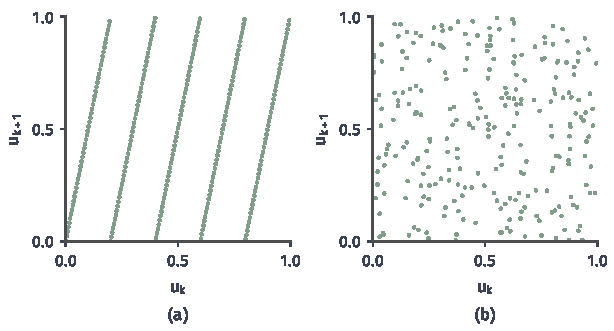
\includegraphics[width=104mm]{figures/07-probability/08-sampling-and-integration/matplotlib/sgen-lcg-pairs/figure.pdf}
  \caption{相邻伪随机数$(u_k,u_{k+1})$组成的点。(a)线性同余递推$s_{k+1}=(5s_k+1)\bmod256$，种子$s_0=7$，一个完整周期的$256$个点全部落在斜率为$5$的五条线段上；(b)NumPy的PCG64生成器，种子$7$，$256$对数。两者的单个$u_k$都在$[0,1)$上均匀分布，差别只在相邻数的联合分布上。}
  \label{fig:sgen-lcg-pairs}
\end{BookInlineFigure}

实用的生成器周期极长（例如$2^{128}$量级），并通过了大量针对相邻数、长程相关和高维分布的统计检验\scite{math-knuth1997seminumerical}。检验通过只说明没有发现所测试的那类偏差，并不证明序列与理想模型无法区分。本卷此后的推导都在理想模型下进行，把“伪随机数足够接近理想模型”当作一个外部假设。

\paragraph{种子与复现}
固定种子，同一程序就产生同一串数，整个计算可以逐位复现。这对查错和比较方法很有用：改动一处代码后用同一种子重跑，结果的变化只来自改动本身。本卷图中的模拟都注明了种子。

复现不等于验证。一个错误的生成方法在固定种子下同样给出可复现的错误结果；某个种子下直方图“看起来对”，换一个种子也可能仍然看起来对，因为错误可能只出现在很少被抽到的区域。生成方法是否正确，要靠式~\eqref{eq:sgen-correct-law}那样的证明，再加上第~\ref{sec:sgen-checks}节的检查；种子只负责让计算可以重来一遍。

\paragraph{有限精度}
浮点数格式也会改变理想模型。常见的双精度均匀数取值于$\{k2^{-53}:k=0,1,\dots,2^{53}-1\}$，可能取到$0$，取不到$1$。若后续要计算$\ln u$，取到$0$就会出错，所以要先确认生成器的取值范围，必要时改用$1-u$。格点还截断了尾部：由$-\ln(1-u)$生成的指数样本不会超过$53\ln2\approx36.7$。对指数分布，被截去的概率约为$\mathrm{e}^{-36.7}$，可以忽略；对尾部很重的分布或专门研究稀有事件的计算，这种截断就需要单独检查。

\section{变量变换构造}
\label{sec:sgen-transform}

最直接的生成方式是找一个确定的映射$T$，把一个容易抽取的变量$V$（通常是若干个基础随机数）变成目标样本$X=T(V)$。这一步本身没有随机性，所有随机性都来自$V$。要说明它正确，就是要算出$T(V)$的分布并与目标比较。

\paragraph{输出分布的两种算法}
$T(V)$的分布是$V$的分布在$T$下的推前：对目标空间的事件$A$，
\[
  \mathbb{P}\bigl(T(V)\in A\bigr)=\mathbb{P}\bigl(V\in T^{-1}(A)\bigr).
\]
这是第~\ref{chap:probability-spaces}章的原像规则，它对任何可测映射成立，不要求$T$可逆，也不要求输出有密度。另一种算法是第~\ref{chap:random-variable-transformations}章的换元公式：若$V$在开集$D\subset\mathbb{R}^{d}$上有密度$f_V$，$T$把$D$一一地映到$T(D)$，连续可微且Jacobian行列式处处非零，记逆映射为$h=T^{-1}$，则$X$有密度
\begin{equation}
  f_X(x)=f_V\bigl(h(x)\bigr)\,\bigl\lvert\det Dh(x)\bigr\rvert,\qquad x\in T(D),
  \label{eq:sgen-change-of-variables}
\end{equation}
在$T(D)$之外为零。换元公式把“质量守恒”写成密度的形式：$x$附近的小体积元来自$h(x)$附近的体积元，体积按$\lvert\det Dh\rvert$倍伸缩，密度按反比变化。

\paragraph{一个用换元公式验证的例子}
取两个独立的基础随机数$(U_1,U_2)$，令
\begin{equation}
  Z_1=\sqrt{-2\ln U_1}\,\cos(2\pi U_2),\qquad Z_2=\sqrt{-2\ln U_1}\,\sin(2\pi U_2).
  \label{eq:sgen-box-muller}
\end{equation}
这称为\term{Box--Muller变换}（Box--Muller transform）。它的想法来自第~\ref{chap:random-variable-transformations}章的极坐标计算：二维标准高斯向量的半径与角度独立，角度均匀，半径平方服从$\operatorname{Exp}(1/2)$。式~\eqref{eq:sgen-box-muller}把$U_2$变成均匀角度$2\pi U_2$，把$U_1$变成半径$R=\sqrt{-2\ln U_1}$。半径平方的分布正是所需的指数分布：对$s>0$，
\[
  \mathbb{P}(R^{2}>s)=\mathbb{P}\bigl(U_1<\mathrm{e}^{-s/2}\bigr)=\mathrm{e}^{-s/2}.
\]

下面用式~\eqref{eq:sgen-change-of-variables}直接验证。$T$把正方形$D=(0,1)^{2}$一一地映到平面去掉非负$z_1$半轴后的区域：半径$r=\sqrt{-2\ln u_1}$取遍$(0,\infty)$，角度$\theta=2\pi u_2$取遍$(0,2\pi)$。记$r^{2}=z_1^{2}+z_2^{2}$，$\theta(z)$为$(z_1,z_2)$在$(0,2\pi)$内的极角，逆映射是
\[
  h(z_1,z_2)=\Bigl(\mathrm{e}^{-r^{2}/2},\ \frac{\theta(z)}{2\pi}\Bigr).
\]
第一个分量对$z_1,z_2$的偏导数分别是$-z_1\mathrm{e}^{-r^{2}/2}$与$-z_2\mathrm{e}^{-r^{2}/2}$；由$\partial\theta/\partial z_1=-z_2/r^{2}$、$\partial\theta/\partial z_2=z_1/r^{2}$，第二个分量的偏导数是$-z_2/(2\pi r^{2})$与$z_1/(2\pi r^{2})$。于是
\[
  \det Dh=-z_1\mathrm{e}^{-r^{2}/2}\cdot\frac{z_1}{2\pi r^{2}}-\Bigl(-z_2\mathrm{e}^{-r^{2}/2}\Bigr)\Bigl(-\frac{z_2}{2\pi r^{2}}\Bigr)=-\frac{\mathrm{e}^{-r^{2}/2}}{2\pi}.
\]
$f_V\equiv1$，代入式~\eqref{eq:sgen-change-of-variables}，得到
\[
  f_Z(z_1,z_2)=\frac{1}{2\pi}\mathrm{e}^{-(z_1^{2}+z_2^{2})/2}=\varphi(z_1)\,\varphi(z_2).
\]
被去掉的半轴面积为零，不影响分布。密度分解为两个标准高斯密度的乘积，所以$Z_1,Z_2$独立，都服从$\mathcal{N}(0,1)$。

用$u_1=0.37$、$u_2=0.80$走一遍：
\[
  r=\sqrt{-2\ln0.37}\approx1.4101,\qquad 2\pi u_2=1.6\pi,
\]
于是
\[
  z_1=1.4101\cos(1.6\pi)\approx0.4358,\qquad z_2=1.4101\sin(1.6\pi)\approx-1.3411.
\]

\paragraph{不需要密度的情形}
换元公式只适用于同维、一一、可微的映射。很多生成映射不满足这些条件，这时直接用原像规则。例如$X=\max\{U_1,U_2\}$把二维变成一维，对$0\le x\le1$，
\[
  \mathbb{P}(X\le x)=\mathbb{P}(U_1\le x,\ U_2\le x)=x^{2},
\]
所以$X$的密度是$2x$。又如下一小节的离散生成，输出只取有限个值，根本没有密度；奇异协方差的高斯生成，输出落在一个低维子空间上，在整个空间中也没有密度。这些情形的输出分布照样由推前确定，正确性同样由式~\eqref{eq:sgen-correct-law}检验。

\subsection{逆分位数采样}
\label{sec:sgen-inverse}

一维的目标分布由分布函数$F$完全确定。对一个均匀数$u$，能否找一个点$x$使“$F$在$x$处恰好累积到$u$”？这就是取分位数。第~\ref{chap:random-variables}章定义了分位数函数
\begin{equation}
  Q(u)=\inf\{x\in\mathbb{R}:F(x)\ge u\},\qquad 0<u<1,
  \label{eq:sgen-quantile}
\end{equation}
并证明了对一切实数$x$，$Q(u)\le x$当且仅当$u\le F(x)$。

\paragraph{方法与正确性}
把基础随机数代入分位数函数，令$X=Q(U)$。由上面的等价关系，
\[
  \mathbb{P}(X\le x)=\mathbb{P}\bigl(U\le F(x)\bigr)=F(x),
\]
所以$X$的分布函数就是$F$。第~\ref{chap:random-variables}章与第~\ref{chap:probability-spaces}章已经从两个角度证明了这一结论，这里关心的是怎样把它变成计算。这种方法称为\term{逆变换采样}（inverse transform sampling）。它对一切实值分布成立：离散、连续或二者混合，有没有密度都一样。几何上，在分布函数的图上从纵轴高度$u$水平向右，碰到曲线（或跳跃的竖直段）后竖直落下，落点就是样本。

\paragraph{分位数有解析式}
若$F$连续且严格递增，$Q$就是$F$的反函数，解方程$F(x)=u$即可。指数分布$\operatorname{Exp}(\lambda)$的$F(x)=1-\mathrm{e}^{-\lambda x}$，解得
\begin{equation}
  Q(u)=-\frac{\ln(1-u)}{\lambda}.
  \label{eq:sgen-exp-quantile}
\end{equation}
取$\lambda=2$、$u=0.37$，得到
\[
  x=-\frac{\ln0.63}{2}\approx\frac{0.4620}{2}=0.2310.
\]
因为$1-U$也服从$\operatorname{Unif}(0,1)$，实际计算中常把式~\eqref{eq:sgen-exp-quantile}换成$-\ln U/\lambda$，省去一次减法；这时需要$U$取不到$0$。

\paragraph{离散分布与累计区间}
设$X$取值$x_1<x_2<\dots<x_K$，概率为$p_1,\dots,p_K$。记累计概率$c_0=0$、$c_k=p_1+\dots+p_k$。此时$F$是阶梯函数，由式~\eqref{eq:sgen-quantile}，$Q(u)=x_k$当且仅当$c_{k-1}<u\le c_k$。也就是说，把$(0,1)$按顺序切成长度为$p_1,\dots,p_K$的区间，$u$落进第$k$段就输出$x_k$：
\begin{equation}
  X=x_k\quad\Longleftrightarrow\quad c_{k-1}<U\le c_k .
  \label{eq:sgen-discrete-inverse}
\end{equation}
每段的长度正好是对应的概率，这一点不用分位数的语言也能看出。

以$\{1,2,3\}$上的分布$p=(0.2,0.5,0.3)$为例，累计概率是
\[
  c_1=0.2,\qquad c_2=0.7,\qquad c_3=1 .
\]
$u=0.37$落在$(0.2,0.7]$，输出$2$；$u=0.85$落在$(0.7,1]$，输出$3$。图~\ref{fig:sgen-discrete-inverse}(a)在分布函数上画出这两次查找：水平线碰到跳跃的竖直段，跳跃的高度就是那个值的概率。(b)是用$1000$个基础随机数生成的样本频率，与真实概率相差都在$0.03$以内。

\begin{BookInlineFigure}
  \centering
  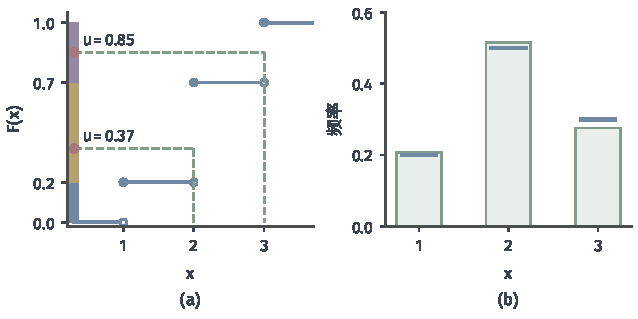
\includegraphics[width=108mm]{figures/07-probability/08-sampling-and-integration/matplotlib/sgen-discrete-inverse/figure.pdf}
  \caption{离散分布$p=(0.2,0.5,0.3)$的逆变换采样。(a)蓝线是分布函数，纵轴上的蓝、黄、紫三段是累计区间$(0,0.2]$、$(0.2,0.7]$、$(0.7,1]$；绿色虚线从$u=0.37$与$u=0.85$出发，分别落到$2$和$3$。(b)绿色柱是$1000$个样本（种子$11$）的频率$0.208,0.516,0.276$，蓝色短横线是真实概率。}
  \label{fig:sgen-discrete-inverse}
\end{BookInlineFigure}

式~\eqref{eq:sgen-discrete-inverse}的计算量在于找到$u$落在哪一段。从$k=1$起逐段比较，需要比较的次数是$X$对应的下标$k$，平均$\sum_kkp_k$次；例中为$0.2+1.0+0.9=2.1$次。若先把各值按概率从大到小排列，同一分布的平均次数降为$1\cdot0.5+2\cdot0.3+3\cdot0.2=1.7$次。$K$很大时，可以预先存好累计概率，用二分查找，每次约$\log_2K$次比较。

含原子的连续分布也由同一公式处理。分布函数在原子处的跳跃，对应$Q$的一段水平平台：长度等于原子概率的一段$u$全部被送到同一个点。第~\ref{chap:probability-spaces}章的等待时间在$0$处有概率$0.3$的原子，$u\le0.3$时输出$0$，就是这种情形。

\paragraph{需要数值反演的情形}
很多分布的$F$可以计算，$Q$却没有解析式。例如$\operatorname{Gamma}(2,1)$的分布函数是
\begin{equation}
  F(x)=1-(1+x)\mathrm{e}^{-x},\qquad x\ge0,
  \label{eq:sgen-gamma2-cdf}
\end{equation}
方程$F(x)=u$解不出初等的$x$。这时只能用数值方法近似求$Q(u)$。最稳妥的是二分法，它只用到$F$的单调性和式~\eqref{eq:sgen-quantile}的等价关系。

二分法的依据是：对任意点$m$，判断$F(m)\ge u$是否成立，就知道$Q(u)\le m$还是$Q(u)>m$。若已知$Q(u)$落在区间$(a,b]$中，取中点$m=(a+b)/2$做一次判断，就能把区间缩小一半，同时保持“$Q(u)$在区间内”这一事实。$k$轮后区间长度为$(b-a)/2^{k}$，输出中点，误差不超过区间长度的一半。

\needspace{6\baselineskip}
\paragraph{变量}
\begin{itemize}
  \item $u\in(0,1)$：基础随机数，整个过程中不变。
  \item $a<b$：当前区间的端点，始终满足$F(a)<u\le F(b)$，于是$Q(u)\in(a,b]$。
  \item $m$：当前区间的中点。
\end{itemize}

\paragraph{初始化}
取一个区间$(a,b]$，使$F(a)<u\le F(b)$。例中取$u=0.37$，$a=0$，$b=8$，因为
\[
  F(0)=0<0.37,\qquad F(8)=1-9\mathrm{e}^{-8}\approx0.9970\ge0.37 .
\]

\needspace{6\baselineskip}
\paragraph{每轮更新}
\begin{enumerate}
  \item \textbf{取中点。}令$m=(a+b)/2$，计算$F(m)$。例中第一轮$m=4$，由式~\eqref{eq:sgen-gamma2-cdf}，
  \[
    F(4)=1-5\mathrm{e}^{-4}\approx0.9084 .
  \]
  \item \textbf{缩小区间。}若$F(m)\ge u$，则$Q(u)\le m$，令$b\leftarrow m$；否则$Q(u)>m$，令$a\leftarrow m$。例中$0.9084\ge0.37$，区间变为$(0,4]$。

  以后各轮的中点、函数值和新区间依次为
  \[
    \begin{aligned}
      m&=2,& F(2)&\approx0.5940,& &(0,2];\\
      m&=1,& F(1)&\approx0.2642,& &(1,2];\\
      m&=1.5,& F(1.5)&\approx0.4422,& &(1,1.5];\\
      m&=1.25,& F(1.25)&\approx0.3554,& &(1.25,1.5].
    \end{aligned}
  \]
  \item \textbf{停止。}区间长度不超过预先给定的$2\delta$时停止，输出中点。例中取$\delta=0.125$，第五轮后长度为$0.25$，停止。
\end{enumerate}
最终输出$\widetilde{x}=1.375$。用更多轮次算出的真值是$Q(0.37)\approx1.2910$，误差约$0.084$，在$\delta=0.125$以内。图~\ref{fig:sgen-bisection-inverse}(a)画出了五个中点。

\paragraph{反演误差怎样改变输出分布}
数值反演输出的不是$Q(U)$，而是近似值$\widetilde{X}=\widetilde{Q}(U)$。它的分布已经不是$F$，问题是偏差多大。下面的引理把每个$u$上的反演误差转成分布函数的偏差。

\begin{lemma}[反演误差的传递]
\label{lem:sgen-inversion-error}
设$\delta\ge0$，函数$\widetilde{Q}$对一切$u\in(0,1)$满足$\lvert\widetilde{Q}(u)-Q(u)\rvert\le\delta$。记$\widetilde{F}$为$\widetilde{X}=\widetilde{Q}(U)$的分布函数，则对一切实数$x$，
\begin{equation}
  F(x-\delta)\le\widetilde{F}(x)\le F(x+\delta).
  \label{eq:sgen-inversion-band}
\end{equation}
若$F$还有不超过$L$的密度，则$\sup_x\lvert\widetilde{F}(x)-F(x)\rvert\le L\delta$。
\end{lemma}

\begin{proof}
若$\widetilde{X}\le x$，则$Q(U)\le\widetilde{X}+\delta\le x+\delta$，所以事件$\{\widetilde{X}\le x\}$包含于$\{Q(U)\le x+\delta\}$。取概率，由$Q(U)$的分布函数是$F$，得$\widetilde{F}(x)\le F(x+\delta)$。

反过来，若$Q(U)\le x-\delta$，则$\widetilde{X}\le Q(U)+\delta\le x$，所以$\{Q(U)\le x-\delta\}$包含于$\{\widetilde{X}\le x\}$，取概率得$F(x-\delta)\le\widetilde{F}(x)$。

若密度不超过$L$，则$F(x+\delta)-F(x)\le L\delta$，$F(x)-F(x-\delta)\le L\delta$，代入式~\eqref{eq:sgen-inversion-band}即得最后一句。
\end{proof}

引理的条件是“对所有$u$都有误差界$\delta$”，这一条在实际中容易被破坏。上面的二分法从固定区间$(0,8]$出发，当$u>F(8)\approx0.9970$时$Q(u)>8$，初始化条件不成立，二分法的每一轮都把区间推向右端，最终输出$7.875$，误差可以任意大。于是约$0.3\%$的尾部质量被搬到了$7.875$这一个点上。要保住误差界，初始化时须先把$b$向右扩大到$F(b)\ge u$为止。

即使误差界成立，输出的分布形状也可能改变。固定做五轮二分时，输出总是某个长$0.25$的小区间的中点，$\widetilde{X}$只取有限个值，是离散分布。图~\ref{fig:sgen-bisection-inverse}(b)画出它的分布函数：一条阶梯，夹在式~\eqref{eq:sgen-inversion-band}的两条紫色虚线之间。$\operatorname{Gamma}(2,1)$的密度$x\mathrm{e}^{-x}$的最大值是$\mathrm{e}^{-1}\approx0.368$，按引理，分布函数的偏差不超过$0.368\times0.125\approx0.046$；数值计算的最大偏差约为$0.0456$。用这样的样本估计依赖于细小尺度的量（例如落在某个短区间内的概率），偏差会比估计期望时明显。

\begin{BookInlineFigure}
  \centering
  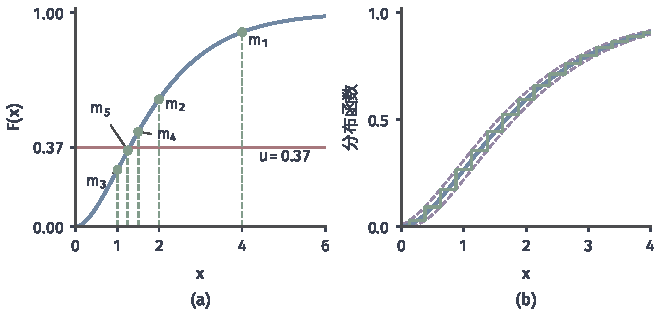
\includegraphics[width=112mm]{figures/07-probability/08-sampling-and-integration/matplotlib/sgen-bisection-inverse/figure.pdf}
  \caption{用二分法数值反演$\operatorname{Gamma}(2,1)$的分布函数。(a)蓝线是$F(x)=1-(1+x)\mathrm{e}^{-x}$，红线是$u=0.37$，绿点是五轮的中点$m_1,\dots,m_5=4,2,1,1.5,1.25$，最后区间为$(1.25,1.5]$。(b)固定做五轮时输出的分布函数（绿色阶梯）与$F$（蓝线），紫色虚线是$F(x-0.125)$与$F(x+0.125)$，阶梯始终夹在两者之间。}
  \label{fig:sgen-bisection-inverse}
\end{BookInlineFigure}

二分法每轮把误差减半，达到$\delta$需要约$\log_2((b-a)/\delta)$次分布函数求值。若$F$有可以计算的密度$f$，也可以用Newton迭代$x\leftarrow x-(F(x)-u)/f(x)$，在解附近每轮有效数字约翻一倍，但初值不好时可能越出定义域，常与二分法配合使用。不论用哪种方法，停止规则给出的误差界都要对全部$u$成立，引理~\ref{lem:sgen-inversion-error}才能用来估计输出分布的偏差。

\subsection{高斯样本生成}
\label{sec:sgen-gaussian}

高斯分布是最常用的目标，它的生成分两步：先生成独立的标准高斯坐标，再用一个仿射变换调出指定的均值与协方差。

\paragraph{独立标准高斯坐标}
标准高斯的分布函数$\Phi$连续且严格递增，由逆变换采样，$Z=\Phi^{-1}(U)$服从$\mathcal{N}(0,1)$。$\Phi^{-1}$没有初等表达式，常用的数值程序以有理函数逼近，在双精度下的误差已接近舍入误差，按引理~\ref{lem:sgen-inversion-error}，对输出分布的影响可以忽略。对$d$个相互独立的基础随机数分别作变换，
\[
  Z_j=\Phi^{-1}(U_j),\qquad j=1,\dots,d,
\]
各$Z_j$是不同基础随机数的函数，所以相互独立，组成的向量$\bm{Z}$服从$\mathcal{N}(\bm{0},\bm{I})$。式~\eqref{eq:sgen-box-muller}是另一种办法，每两个基础随机数给出两个独立的标准高斯数，只用到对数与三角函数。

例如取$u_1=0.37$、$u_2=0.80$，
\[
  z_1=\Phi^{-1}(0.37)\approx-0.3319,\qquad z_2=\Phi^{-1}(0.80)\approx0.8416 .
\]

\paragraph{仿射变换}
要生成$\mathcal{N}(\bm{\mu},\bm{\Sigma})$，其中$\bm{\mu}\in\mathbb{R}^{d}$是均值向量，$\bm{\Sigma}\in\mathbb{R}^{d\times d}$是对称半正定的协方差矩阵，先把$\bm{\Sigma}$分解为
\begin{equation}
  \bm{\Sigma}=\bm{A}\bm{A}^{\top},\qquad \bm{A}\in\mathbb{R}^{d\times r},
  \label{eq:sgen-cov-factor}
\end{equation}
再取$r$个独立标准高斯坐标组成$\bm{Z}$，令
\begin{equation}
  \bm{X}=\bm{\mu}+\bm{A}\bm{Z}.
  \label{eq:sgen-gaussian-affine}
\end{equation}
由期望的线性，$\mathbb{E}[\bm{X}]=\bm{\mu}$；由协方差在线性变换下的规则，
\[
  \operatorname{Cov}(\bm{X})=\bm{A}\operatorname{Cov}(\bm{Z})\bm{A}^{\top}=\bm{A}\bm{I}\bm{A}^{\top}=\bm{\Sigma}.
\]
第~\ref{chap:multivariate-distributions}章正是用这种形式定义多元高斯分布的，并证明了$\bm{\mu}+\bm{A}\bm{Z}$的分布只依赖于$\bm{A}\bm{A}^{\top}$，所以不论选哪个因子，都有$\bm{X}\sim\mathcal{N}(\bm{\mu},\bm{\Sigma})$。这一论证没有用到密度，因而不要求$\bm{\Sigma}$可逆。

因子$\bm{A}$有两种常用取法。$\bm{\Sigma}$正定时，Cholesky分解给出对角元为正的下三角矩阵$\bm{L}$，使$\bm{\Sigma}=\bm{L}\bm{L}^{\top}$，计算量约为$d^{3}/3$次乘法（可参考\BookChapterRef{chap:direct-linear-solvers}{卷二第12章“线性方程的直接求解”}）。$\bm{\Sigma}$只是半正定时，Cholesky分解会遇到零主元，可改用谱分解$\bm{\Sigma}=\bm{V}\bm{\Lambda}\bm{V}^{\top}$（可参考\BookChapterRef{chap:eigen-spectral-decomposition}{卷二第6章“谱分解”}），取$\bm{A}=\bm{V}\bm{\Lambda}^{1/2}$，并去掉特征值为零的列。分解只需做一次，之后每个样本只需$d$个标准高斯数和一次矩阵乘向量。

用一个二维例子走一遍。取
\[
  \bm{\mu}=\begin{bmatrix}1\\0\end{bmatrix},\qquad
  \bm{\Sigma}=\begin{bmatrix}4&2\\2&2\end{bmatrix},\qquad
  \bm{L}=\begin{bmatrix}2&0\\1&1\end{bmatrix},
\]
可以直接验证$\bm{L}\bm{L}^{\top}=\bm{\Sigma}$。代入上面的$z_1,z_2$，由式~\eqref{eq:sgen-gaussian-affine}，
\[
  \bm{x}=\begin{bmatrix}1+2z_1\\ z_1+z_2\end{bmatrix}\approx\begin{bmatrix}0.3363\\0.5098\end{bmatrix}.
\]
下三角结构使第一个坐标只用到$z_1$，第二个坐标用到$z_1$和$z_2$；两个坐标共用$z_1$，这正是它们的协方差$2$的来源。

\paragraph{奇异协方差}
若$\bm{\Sigma}$的秩$r<d$，式~\eqref{eq:sgen-gaussian-affine}仍然给出正确的分布，但$\bm{X}-\bm{\mu}=\bm{A}\bm{Z}$总落在$\bm{A}$的列空间中，这是一个$r$维子空间。例如
\[
  \bm{\Sigma}=\begin{bmatrix}1&2\\2&4\end{bmatrix}=\bm{a}\bm{a}^{\top},\qquad \bm{a}=\begin{bmatrix}1\\2\end{bmatrix},
\]
只需一个标准高斯数，$\bm{X}=\bm{\mu}+Z_1\bm{a}$全部落在过$\bm{\mu}$、方向为$\bm{a}$的直线上。这条直线在平面上的面积为零，$\bm{X}$在$\mathbb{R}^{2}$中没有密度，式~\eqref{eq:sgen-change-of-variables}无从使用；推前的论证不受影响。图~\ref{fig:sgen-gaussian-affine}对比了三种情形。

\begin{BookInlineFigure}
  \centering
  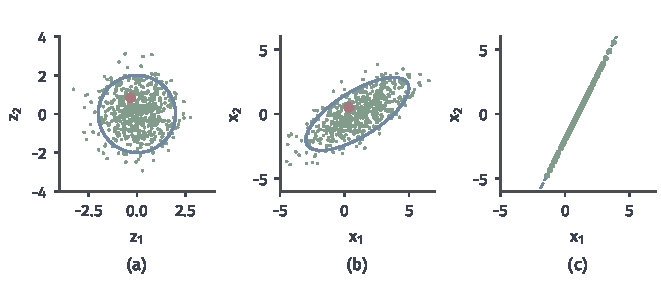
\includegraphics[width=112mm]{figures/07-probability/08-sampling-and-integration/matplotlib/sgen-gaussian-affine/figure.pdf}
  \caption{由独立标准高斯坐标生成指定协方差的高斯样本，$600$个样本（种子$5$）。(a)标准高斯$\bm{Z}$，蓝线是半径$2$的圆，红点是$(\Phi^{-1}(0.37),\Phi^{-1}(0.80))$；(b)$\bm{X}=\bm{\mu}+\bm{L}\bm{Z}$，$\bm{\mu}=(1,0)^{\top}$，$\bm{\Sigma}=\bm{L}\bm{L}^{\top}$，圆被变成椭圆，红点是例中的$(0.336,0.510)$；(c)秩为$1$的$\bm{\Sigma}=\bm{a}\bm{a}^{\top}$，样本全部落在蓝色虚线上。}
  \label{fig:sgen-gaussian-affine}
\end{BookInlineFigure}

奇异协方差在数值上还有一个隐患。若$\bm{\Sigma}$本应奇异，由于舍入它的最小特征值可能算成很小的负数，Cholesky分解随之失败；若$\bm{\Sigma}$本应正定但极接近奇异，分解得到的因子误差也会很大。谱分解可以把很小的负特征值截为零，但截断改变了协方差，偏差的大小应与$\bm{\Sigma}$的元素尺度一起报告。

\section{分步生成}
\label{sec:sgen-sequential}

有些目标分布找不到一个简单的整体映射，却可以拆成几个容易处理的部分。混合分布可以拆成“选哪一个成分”和“在成分内抽样”；多维分布可以按链式分解拆成“先抽第一个坐标，再按条件分布抽下一个坐标”。分步生成就是按这种拆分依次抽取，每一步只需要一个简单的生成方法。

检验分步生成是否正确，用的是全概率公式与链式分解：各步的分布按顺序拼起来，应当恰好拼回目标分布。拼接成立的前提是：每一步都取新的基础随机数，与前面各步用过的互不重叠。要注意这里的独立指的是输入：各步的基础随机数独立，并不意味着同一个样本的各个坐标独立，后一步的输出通常依赖前一步的输出。

\subsection{混合分布采样}
\label{sec:sgen-mixture}

设目标是有限混合
\begin{equation}
  \pi=\sum_{k=1}^{K}w_kP_k,\qquad w_k\ge0,\quad \sum_{k=1}^{K}w_k=1,
  \label{eq:sgen-mixture}
\end{equation}
其中每个成分$P_k$都能直接生成。全章的例子$0.3\,\mathcal{N}(-2,0.5^{2})+0.7\,\mathcal{N}(2,1)$就是这样：两个成分都是高斯分布，混合后却有两个峰，没有简单的分位数公式。

\paragraph{方法}
混合分布的意思是“先按权重选一个成分，再从这个成分中抽样”。按这个描述，用一个基础随机数$U_0$按累计权重$c_k=w_1+\dots+w_k$选出成分编号
\[
  J=k\quad\Longleftrightarrow\quad c_{k-1}<U_0\le c_k ,
\]
这正是式~\eqref{eq:sgen-discrete-inverse}；再用另一组基础随机数$\bm{U}'$生成$X=G_J(\bm{U}')$，其中$G_k$是第$k$个成分的生成方法。这种分步构造也称为\term{复合法}（composition method）。

\begin{theorem}[混合分布采样]
\label{thm:sgen-mixture}
设$U_0$与$\bm{U}'$独立，$\mathbb{P}(J=k)=w_k$，且对每个$k$，$G_k(\bm{U}')$的分布是$P_k$。则$X=G_J(\bm{U}')$的分布是式~\eqref{eq:sgen-mixture}中的$\pi$。
\end{theorem}

\begin{proof}
对任意事件$A$，按成分编号分解，
\[
  \mathbb{P}(X\in A)=\sum_{k=1}^{K}\mathbb{P}\bigl(J=k,\ G_k(\bm{U}')\in A\bigr).
\]
$J$只依赖$U_0$，$G_k(\bm{U}')$只依赖$\bm{U}'$，二者独立，所以每一项分解为乘积，
\[
  \mathbb{P}(X\in A)=\sum_{k=1}^{K}\mathbb{P}(J=k)\,\mathbb{P}\bigl(G_k(\bm{U}')\in A\bigr)=\sum_{k=1}^{K}w_kP_k(A)=\pi(A). \qedhere
\]
\end{proof}

这就是全概率公式：$J$把样本空间分成$K$块，每块内的条件分布是$P_k$。用例子走一遍：累计权重$c_1=0.3$、$c_2=1$，取$u_0=0.37>0.3$，选第二个成分；再取$u_1=0.80$，由逆变换得$\Phi^{-1}(0.80)\approx0.8416$，于是
\[
  x=2+1\times0.8416=2.8416 .
\]
生成一个样本用了两个基础随机数：一个选成分，一个在成分内生成。一般地，用量是$1$加上所选成分的用量，平均为$1+\sum_kw_k\,(\text{第}k\text{个成分的用量})$。

\paragraph{共用随机数会怎样}
定理~\ref{thm:sgen-mixture}的证明中，唯一用到的性质是$J$与$\bm{U}'$独立。若为了省一个随机数，让同一个$U$既选成分又在成分内生成，即$X=m_J+s_J\Phi^{-1}(U)$，结论就不再成立。$U\le0.3$时选第一个成分，但此时$\Phi^{-1}(U)\le\Phi^{-1}(0.3)$，只能得到第一个成分的下方$30\%$；$U>0.3$时只能得到第二个成分的上方$70\%$。计算可得，输出在$x\le-2+0.5\,\Phi^{-1}(0.3)\approx-2.262$上的密度是$\varphi((x+2)/0.5)/0.5$，在$x>2+\Phi^{-1}(0.3)\approx1.476$上的密度是$\varphi(x-2)$，中间没有质量。各成分的总权重仍然是$0.3$和$0.7$，形状却完全错了。图~\ref{fig:sgen-mixture}对比了两种做法。

\begin{BookInlineFigure}
  \centering
  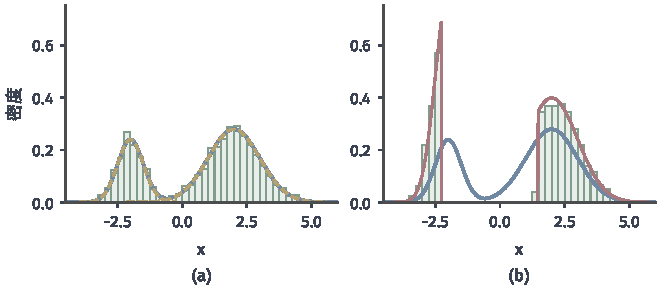
\includegraphics[width=112mm]{figures/07-probability/08-sampling-and-integration/matplotlib/sgen-mixture/figure.pdf}
  \caption{混合分布$0.3\,\mathcal{N}(-2,0.5^{2})+0.7\,\mathcal{N}(2,1)$的分步生成，$4000$个样本（种子$3$）。(a)选成分与成分内生成使用独立的基础随机数，绿色直方图与蓝色目标密度吻合，黄色虚线是两个加权成分；(b)同一个$U$同时用于两步，直方图只覆盖第一个成分的左侧与第二个成分的右侧，红线是按正文算出的输出密度。}
  \label{fig:sgen-mixture}
\end{BookInlineFigure}

共用随机数并非一定出错，关键在于共用的部分是否仍与$J$独立。令$V=(U-c_{J-1})/w_J$，即把$U$在所选区间内的位置重新拉伸到$(0,1)$。对每个$k$和$0\le v\le1$，
\[
  \mathbb{P}(J=k,\ V\le v)=\mathbb{P}\bigl(c_{k-1}<U\le c_{k-1}+w_kv\bigr)=w_kv=\mathbb{P}(J=k)\,v,
\]
所以$V$服从$\operatorname{Unif}(0,1)$且与$J$独立，可以代替$\bm{U}'$使用。代价是精度：$w_k$很小时，$V$只继承了$U$的少数几位有效数字，在有限精度下取值很稀疏。除非随机数生成确实是瓶颈，否则直接取新的基础随机数更简单。

\paragraph{连续混合}
混合的成分编号也可以是连续参数。若$\pi(A)=\int P_{\theta}(A)\,\nu(\mathrm{d}\theta)$，就先按$\nu$抽出$\theta$，再按$P_{\theta}$抽$X$，证明与定理~\ref{thm:sgen-mixture}相同，只是求和换成积分。第~\ref{chap:multivariate-distributions}章的正态尺度混合就是一例：先抽$W\sim\operatorname{Gamma}(\nu/2,\nu/2)$，再抽$X\sim\mathcal{N}(0,1/W)$，得到的$X$服从$t_{\nu}$。

\subsection{按条件分布生成坐标}
\label{sec:sgen-ancestral}

多维目标往往没有整体的生成映射，但它的联合分布可以按坐标依次分解。设$\bm{X}=(X_1,\dots,X_d)$的联合分布写成
\begin{equation}
  \pi(\mathrm{d}x_1,\dots,\mathrm{d}x_d)=P_1(\mathrm{d}x_1)\,K_2(x_1,\mathrm{d}x_2)\cdots K_d(x_{1:d-1},\mathrm{d}x_d),
  \label{eq:sgen-chain-decomposition}
\end{equation}
其中$P_1$是$X_1$的边缘分布，$K_j(x_{1:j-1},\cdot)$是给定前$j-1$个坐标时$X_j$的条件分布，$x_{1:j-1}$是$(x_1,\dots,x_{j-1})$的简写。第~\ref{chap:conditional-distributions}章证明了，在一般的取值空间上，这样的分解总是存在。生成时只要每个条件分布都能抽样。

\paragraph{方法与正确性}
先用$U_1$生成$X_1\sim P_1$；对$j=2,\dots,d$，用新的基础随机数$U_j$生成
\[
  X_j=G_j(X_{1:j-1},U_j),
\]
其中对每个固定的$x_{1:j-1}$，$G_j(x_{1:j-1},U_j)$的分布是$K_j(x_{1:j-1},\cdot)$。这种按顺序生成坐标的方法称为\term{祖先采样}（ancestral sampling）。

正确性按$j$归纳。设$(X_1,\dots,X_{j-1})$的分布已经是$\pi$的前$j-1$个坐标的边缘分布。$U_j$与$X_{1:j-1}$独立，因为后者只用了$U_1,\dots,U_{j-1}$；给定$X_{1:j-1}=x_{1:j-1}$时$X_j$的条件分布因而就是$G_j(x_{1:j-1},U_j)$的分布，即$K_j(x_{1:j-1},\cdot)$。由第~\ref{chap:conditional-distributions}章“边缘分布与概率核确定联合分布”的结论，$(X_1,\dots,X_j)$的分布是前一步的边缘分布与$K_j$的复合，也就是式~\eqref{eq:sgen-chain-decomposition}的前$j$个因子。$j=d$时得到$\pi$。

\paragraph{二元高斯的例子}
取标准化的二元高斯，相关系数$\rho=0.8$：
\[
  \bm{X}\sim\mathcal{N}\Biggl(\bm{0},\begin{bmatrix}1&\rho\\\rho&1\end{bmatrix}\Biggr).
\]
由第~\ref{chap:multivariate-distributions}章的高斯条件分布，给定$X_1=x_1$时$X_2\sim\mathcal{N}(\rho x_1,1-\rho^{2})$。于是祖先采样为
\begin{equation}
  X_1=\Phi^{-1}(U_1),\qquad X_2=\rho X_1+\sqrt{1-\rho^{2}}\,\Phi^{-1}(U_2).
  \label{eq:sgen-bivariate-ancestral}
\end{equation}
取$u_1=0.37$、$u_2=0.80$，$\sqrt{1-\rho^{2}}=0.6$，得到
\[
  x_1\approx-0.3319,\qquad x_2\approx0.8\times(-0.3319)+0.6\times0.8416\approx0.2395 .
\]
$U_1$与$U_2$独立，但$X_1$与$X_2$的相关系数是$0.8$：第二步把第一步的结果$X_1$作为输入用掉了。式~\eqref{eq:sgen-bivariate-ancestral}其实就是$\bm{\Sigma}$的Cholesky因子作用于$(\Phi^{-1}(U_1),\Phi^{-1}(U_2))$，与第~\ref{sec:sgen-gaussian}节的仿射方法一致。

\paragraph{两种“逐坐标”的区别}
祖先采样每生成一个完整的向量，都从第一个坐标重新开始，并使用一组新的基础随机数。第$i$个向量只用第$i$组随机数，所以各向量相互独立、同分布。另有一种做法看起来相似：手里保留一个完整的状态向量，每次只按“给定其余所有坐标”的条件分布重新抽一个坐标，其余坐标保持不变。这就是第~\ref{sec:sgen-gibbs}节的Gibbs采样。图~\ref{fig:sgen-sequential-scheme}画出两者的数据流。

\begin{BookInlineFigure}
  \centering
  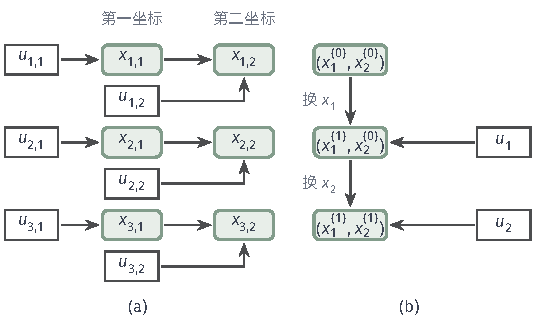
\includegraphics[width=91mm]{figures/07-probability/08-sampling-and-integration/tikz/sgen-sequential-scheme/figure.pdf}
  \caption{两种按坐标生成的数据流，方框是基础随机数，绿色圆角框是生成的坐标或状态。(a)祖先采样：每一行用自己的$u_{i,1},u_{i,2}$从头生成一个向量，行与行之间没有共用的输入；(b)Gibbs采样：保留状态，每次只换一个坐标，相邻状态共用未被更换的坐标。}
  \label{fig:sgen-sequential-scheme}
\end{BookInlineFigure}

两者用到的条件分布也不同。祖先采样需要的是按顺序的条件分布$K_j(x_{1:j-1},\cdot)$，只依赖排在前面的坐标；Gibbs采样需要的是给定其余全部坐标的条件分布。对二元高斯两者都容易得到，但在许多问题中只有后一种可以计算，这时只能退而使用链式更新。代价是：Gibbs采样的相邻状态共用坐标，因而相关，而且一般要从目标分布以外的状态出发。

\section{拒绝采样}
\label{sec:sgen-rejection}

前两节都要求目标分布有可以计算的分位数或可以抽样的分解。很多目标只给出一个密度公式，而且常常只知道到一个常数因子：$\pi(x)=\widetilde{p}(x)/Z$，其中$\widetilde{p}\ge0$可以逐点计算，归一化常数$Z=\int\widetilde{p}(x)\,\mathrm{d}x$却算不出来。模拟退火中的Gibbs分布$\exp(-f(x)/T)/Z_T$就是这样的目标（可参考\BookChapterRef{chap:random-search}{卷五第15章“随机搜索”}），状态多时$Z_T$是一个无法逐项求和的大和式。拒绝采样处理这类目标：从一个容易抽样的\term{建议分布}（proposal distribution）多抽一些候选，再按目标与建议的密度之比筛掉一部分。

这和用随机投点估计面积是同一个想法。在$\widetilde{p}$的图像下方均匀投点，点的横坐标就服从$\pi$；要在图像下方均匀投点，可以先在一个更大、容易投点的区域里均匀投点，再丢掉落在图像上方的点。

\subsection{接受规则的正确性}
\label{sec:sgen-rejection-correct}

设目标的未归一化密度$\widetilde{p}\ge0$满足$0<Z<\infty$；建议分布有密度$q$，可以直接抽样，密度可以计算；存在常数$M>0$，使
\begin{equation}
  \widetilde{p}(x)\le M\,q(x)\qquad\text{对一切}x\text{成立}.
  \label{eq:sgen-envelope}
\end{equation}
$Mq$称为包络，$M$称为\term{包络常数}（envelope constant）。式~\eqref{eq:sgen-envelope}蕴含：凡是$\widetilde{p}(x)>0$的地方都有$q(x)>0$，即建议分布覆盖了目标的全部质量所在。

\paragraph{一次试验}
抽候选$Y\sim q$，再抽与之独立的基础随机数$V$，当
\begin{equation}
  V\le\frac{\widetilde{p}(Y)}{M\,q(Y)}
  \label{eq:sgen-accept-rule}
\end{equation}
时接受$Y$，否则拒绝。$Y$落在$q(Y)=0$处的概率为零，比值总是有定义的；由式~\eqref{eq:sgen-envelope}，比值在$[0,1]$中，可以当作概率。几何上，点$(Y,\,V\,Mq(Y))$在包络$Mq$的图像下方均匀分布，接受规则就是“点落在$\widetilde{p}$的图像下方”。

\begin{theorem}[拒绝采样]
\label{thm:sgen-rejection}
在上述条件下，一次试验的接受概率是
\begin{equation}
  \mathbb{P}(\text{接受})=\frac{Z}{M},
  \label{eq:sgen-acceptance}
\end{equation}
给定接受时$Y$的条件分布是$\pi$。若独立重复试验直到第一次接受，记所用的试验次数为$N$、接受的候选为$X$，则$X\sim\pi$，$N\sim\operatorname{Geom}(Z/M)$，并且$X$与$N$独立。
\end{theorem}

\begin{proof}
对任意事件$A$，先对$Y$取条件，再对$Y$的密度积分。给定$Y=y$，接受的概率是$\widetilde{p}(y)/(Mq(y))$，因为$V$与$Y$独立。于是
\[
  \mathbb{P}(Y\in A,\ \text{接受})=\int_{A}q(y)\,\frac{\widetilde{p}(y)}{M\,q(y)}\,\mathrm{d}y=\frac{1}{M}\int_{A}\widetilde{p}(y)\,\mathrm{d}y=\frac{Z}{M}\,\pi(A).
\]
其中$q(y)=0$的点对积分没有贡献，由式~\eqref{eq:sgen-envelope}，那里$\widetilde{p}(y)=0$。取$A$为全空间，得到式~\eqref{eq:sgen-acceptance}。两式相除，$\mathbb{P}(Y\in A\mid\text{接受})=\pi(A)$。

记$a=Z/M$。各次试验使用互不重叠的基础随机数，相互独立。第$n$次才首次接受且接受的候选落在$A$中，意味着前$n-1$次都拒绝、第$n$次接受且候选在$A$中，所以
\[
  \mathbb{P}(N=n,\ X\in A)=(1-a)^{n-1}\cdot a\,\pi(A).
\]
对$A$取全空间得$\mathbb{P}(N=n)=(1-a)^{n-1}a$，即$N\sim\operatorname{Geom}(a)$；对$n$求和得$\mathbb{P}(X\in A)=\pi(A)$。联合概率等于两者之积，所以$X$与$N$独立。
\end{proof}

定理中各条件的作用如下。$0<Z<\infty$保证$\pi$是概率分布，也保证接受概率为正，否则会无限试下去。式~\eqref{eq:sgen-envelope}保证接受规则中的比值不超过$1$；它一旦失效，正确性随之失效，下面会看到后果。$V$与$Y$独立、各次试验独立，分别用在证明的第一步和第二步。整个算法只用到$\widetilde{p}$，不需要$Z$：$Z$的值只影响接受得多还是少，不影响接受下来的样本的分布。反过来，$M$必须真正满足式~\eqref{eq:sgen-envelope}，这是算法唯一需要预先保证的数。

\needspace{6\baselineskip}
\paragraph{变量}
\begin{itemize}
  \item $y$：当前候选，由建议分布生成。
  \item $v$：与候选配对的基础随机数，用于接受判定。
  \item $n$：已进行的试验次数。
\end{itemize}

\paragraph{初始化}
令$n=0$。下面用的例子是目标$\widetilde{p}(x)=x(1-x)$（$0\le x\le1$），建议分布$q=\operatorname{Unif}(0,1)$。$\widetilde{p}$在$x=1/2$处取最大值$1/4$，所以取$M=1/4$即满足式~\eqref{eq:sgen-envelope}。$Z=\int_0^1x(1-x)\,\mathrm{d}x=1/6$，归一化后$\pi(x)=6x(1-x)$是$\operatorname{Beta}(2,2)$的密度，但算法用不到这两个量。

\needspace{6\baselineskip}
\paragraph{每轮更新}
\begin{enumerate}
  \item \textbf{抽候选。}抽$y\sim q$与基础随机数$v$，令$n\leftarrow n+1$。例中第一轮用两个基础随机数$y=0.9$、$v=0.5$。
  \item \textbf{计算比值。}计算$r=\widetilde{p}(y)/(Mq(y))$。例中第一轮
  \[
    r=\frac{0.9\times0.1}{1/4}=0.36 .
  \]
  \item \textbf{判定。}若$v\le r$，接受$y$并停止；否则回到第1步。例中$0.5>0.36$，拒绝。第二轮取$y=0.37$、$v=0.80$，
  \[
    r=\frac{0.37\times0.63}{1/4}=0.9324\ge0.80,
  \]
  接受。
\end{enumerate}
最终得到样本$x=0.37$，用了$n=2$次试验、$4$个基础随机数。图~\ref{fig:sgen-rejection-envelope}(a)把这两次试验画成点$(y,\,vMq(y))$：$(0.9,0.125)$在抛物线上方，$(0.37,0.2)$在下方。

\begin{BookInlineFigure}
  \centering
  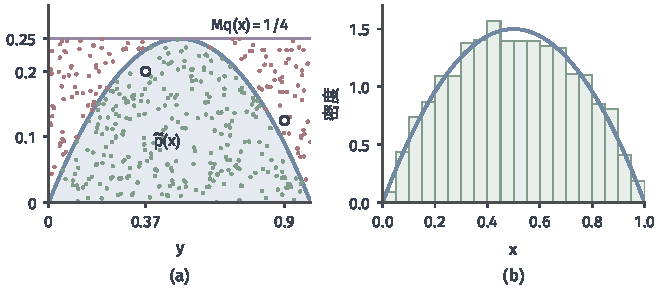
\includegraphics[width=112mm]{figures/07-probability/08-sampling-and-integration/matplotlib/sgen-rejection-envelope/figure.pdf}
  \caption{从$\operatorname{Unif}(0,1)$拒绝采样$\operatorname{Beta}(2,2)$，$\widetilde{p}(x)=x(1-x)$，$M=1/4$。(a)$400$个候选画成点$(y,\,vMq(y))$（种子$2$），紫线是包络$Mq=1/4$，蓝线下方浅蓝区域里的绿点被接受，上方的红点被拒绝；两个空心圆是正文中的两次试验。(b)$6000$个候选中被接受的点的直方图（接受比例$0.6625$），蓝线是$6x(1-x)$。}
  \label{fig:sgen-rejection-envelope}
\end{BookInlineFigure}

\paragraph{包络无效时}
若式~\eqref{eq:sgen-envelope}在某些点不成立，比值$\widetilde{p}/(Mq)$在那里超过$1$，判定$v\le r$必然通过，实际的接受概率是$\min\{1,\widetilde{p}/(Mq)\}$。把定理的第一步计算中的$\widetilde{p}/(Mq)$换成这个量，接受样本的密度正比于
\begin{equation}
  q(x)\min\Bigl\{1,\frac{\widetilde{p}(x)}{M\,q(x)}\Bigr\}=\frac{1}{M}\min\bigl\{\widetilde{p}(x),\,M\,q(x)\bigr\}.
  \label{eq:sgen-invalid-envelope}
\end{equation}
也就是说，目标在包络以上的部分被削平了。在上面的例子中错用$M=1/5$，$x(1-x)>1/5$的区间是$(0.276,0.724)$，输出的密度在这一段变成常数，中部的质量被系统地压低（图~\ref{fig:sgen-rejection-invalid}）。从直方图上看，偏差并不刺眼；程序也不会报错，因为每一步都“正常地”接受或拒绝。所以包络常数必须由推导保证，不能凭几次试算的最大比值来定。

\begin{BookInlineFigure}
  \centering
  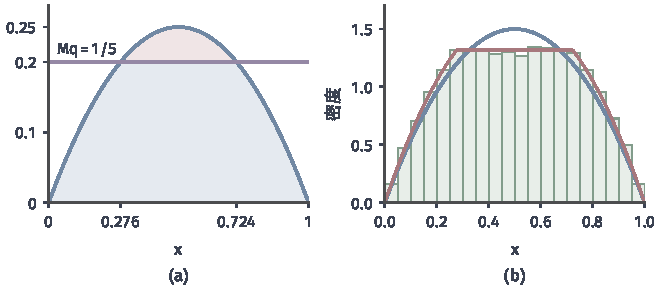
\includegraphics[width=112mm]{figures/07-probability/08-sampling-and-integration/matplotlib/sgen-rejection-invalid/figure.pdf}
  \caption{包络常数过小的后果。(a)蓝线是$\widetilde{p}(x)=x(1-x)$，紫线是错用的$Mq=1/5$，浅红区域是被削去的部分；(b)$20000$个候选中被接受点的直方图（种子$4$），红线是按式~\eqref{eq:sgen-invalid-envelope}归一化的输出密度，蓝线是目标$6x(1-x)$。}
  \label{fig:sgen-rejection-invalid}
\end{BookInlineFigure}

\subsection{接受率与生成成本}
\label{sec:sgen-rejection-cost}

拒绝采样总是正确的，问题在于要试多少次。由定理~\ref{thm:sgen-rejection}，试验次数$N$服从参数为$a=Z/M$的几何分布，于是得到一个样本平均所需的建议次数为
\begin{equation}
  \mathbb{E}[N]=\frac{M}{Z}.
  \label{eq:sgen-expected-trials}
\end{equation}
它就是包络下的面积$M$与目标下的面积$Z$之比，即投点区域中“浪费”的比例的倒数。例中$M/Z=(1/4)/(1/6)=1.5$，平均每个样本要试$1.5$次；图~\ref{fig:sgen-rejection-envelope}(b)中$6000$个候选的接受比例$0.6625$与理论值$2/3$相符。

若$\widetilde{p}=\pi$已经归一化，式~\eqref{eq:sgen-envelope}两边积分得$1\le M$，所以接受率$1/M$不超过$1$，等号当且仅当$q=\pi$（除去零概率集）。包络越贴近目标，$M$越接近$1$。

\paragraph{成本的组成}
一次试验的成本包括生成候选、计算$\widetilde{p}(y)$与$q(y)$、生成$v$。设一次试验的平均成本为$c$，得到$n$个样本的期望成本为$n\,c\,M/Z$，此外还有一次性的准备成本：求出有效的$M$。$M$最好取$\sup_x\widetilde{p}(x)/q(x)$，这需要解一个优化问题；取得太大虽然仍然正确，但成本按比例上升。两种成本的权衡在于：准备工作做一次，试验成本乘以样本数。

试验次数的波动也要计入。$N$的方差是$(1-a)/a^{2}$，接受率低时次数的分布有很长的右尾，生成固定个数的样本所需时间也随之波动。

\paragraph{高维中的接受率}
包络在高维中很难贴紧。设目标是$\mathcal{N}(\bm{0},\bm{I}_d)$，建议分布是$\mathcal{N}(\bm{0},\sigma^{2}\bm{I}_d)$，$\sigma>1$。两个归一化密度之比为
\[
  \frac{\pi(\bm{x})}{q(\bm{x})}=\sigma^{d}\exp\Bigl(-\frac{\lVert\bm{x}\rVert_2^{2}}{2}\bigl(1-\sigma^{-2}\bigr)\Bigr)\le\sigma^{d},
\]
等号在$\bm{x}=\bm{0}$处成立，所以最小的包络常数是$M=\sigma^{d}$，接受率为
\begin{equation}
  a=\sigma^{-d}.
  \label{eq:sgen-acceptance-dimension}
\end{equation}
每个坐标上建议分布只比目标宽一点，接受率也随维数指数下降。$\sigma=1.1$时，$d=10$的接受率约为$0.386$，$d=100$时约为$7.3\times10^{-5}$，平均每个样本要试一万多次。若$\sigma<1$，比值在$\lVert\bm{x}\rVert_2\to\infty$时趋于无穷，根本不存在包络：建议分布的尾部必须不比目标轻。

\begin{BookInlineFigure}
  \centering
  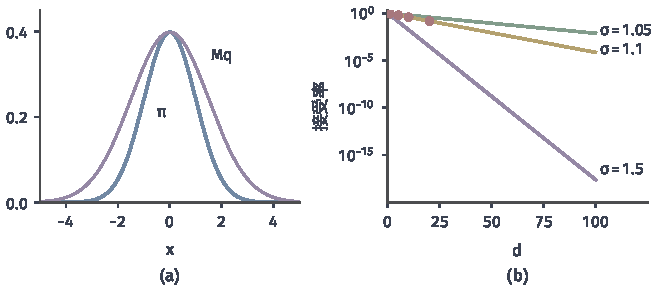
\includegraphics[width=112mm]{figures/07-probability/08-sampling-and-integration/matplotlib/sgen-rejection-dimension/figure.pdf}
  \caption{高斯目标、高斯建议时的拒绝采样。(a)$d=1$、$\sigma=1.5$，蓝线是目标$\pi$，紫线是包络$Mq$，二者只在$x=0$处相切；(b)接受率$\sigma^{-d}$随维数$d$的变化（对数纵轴），绿、黄、紫依次为$\sigma=1.05,1.1,1.5$，红点是$\sigma=1.1$、$d=1,5,10,20$时各$20$万个候选的模拟接受比例（种子$8$）。}
  \label{fig:sgen-rejection-dimension}
\end{BookInlineFigure}

图~\ref{fig:sgen-rejection-dimension}(a)说明了原因：包络只在一点与目标相切，其余地方都留有空隙，空隙所占的比例按维数相乘。一维时浪费不到一半，一百维时几乎全部浪费。拒绝采样在低维、能找到贴身包络的问题中很有效，在高维中通常只作为其他方法的一个组成部分。对那些连有效包络都写不出来的高维目标，需要换一种思路，这就是下一节的链式更新。

\section{MCMC采样}
\label{sec:sgen-mcmc}

直接生成要求一次性造出一个完整的目标样本，这需要分位数、可抽样的分解或贴身的包络。高维目标往往三者都没有，能做的只是逐点计算未归一化密度$\widetilde{p}(x)$，或者计算它的梯度。只靠这些局部信息，能否得到目标分布的样本？

\term{Markov链Monte Carlo}（Markov chain Monte Carlo，MCMC）的回答是：不再从头造样本，而是让一个状态在空间中游走，每一步只根据当前位置随机地走到下一个位置，并设计走法，使目标概率大的地方被访问得更频繁。把目标分布想象成地形的高度，游走者在高处停留得久、在低处停留得短，长时间下来，在各处停留的时间比例就接近目标概率。这个图景有两处需要准确化：“走法不破坏目标分布”是一个可以逐步验证的代数条件，即下面的不变性；“长时间后停留比例接近目标”则还需要链能走遍目标的支持，这是另一个条件，不能由第一个推出。

本节先建立转移与不变分布，再介绍保持目标不变的三种更新，它们分别以Metropolis--Hastings、Gibbs和Hamilton命名。它们的输出都是一串相关的状态，而不是独立样本。

\subsection{转移与不变分布}
\label{sec:sgen-invariance}

\paragraph{转移核}
链式更新的每一步，都是在给定当前状态$x$时，随机地选出下一个状态。把“给定$x$时下一状态的分布”记作$K(x,\cdot)$：对状态空间中的集合$A$，$K(x,A)$是从$x$出发一步后进入$A$的概率。按第~\ref{chap:conditional-distributions}章的定义，$K$是从状态空间到自身的概率核，在这里称为\term{转移核}（transition kernel）。状态有限时，$K$就是一个每行和为$1$的非负矩阵，第$x$行第$y$列为$K(x,\{y\})$。

用转移核生成一条链：给定初始状态$X^{(0)}$，对$t=0,1,2,\dots$，用新的基础随机数从$K(X^{(t)},\cdot)$中抽出$X^{(t+1)}$。具体实现中，常写成$X^{(t+1)}=\Psi(X^{(t)},\bm{U}^{(t+1)})$，其中$\Psi$是确定的更新函数，$\bm{U}^{(t+1)}$是第$t+1$步专用的基础随机数，并且对每个$x$，$\Psi(x,\bm{U})$的分布是$K(x,\cdot)$。由于各步的随机数互不重叠，给定$X^{(t)}$后，$X^{(t+1)}$与更早的状态无关，这正是Markov链的含义，第~\ref{chap:information-measures}章对三个变量用过的Markov性在这里对整个序列成立。

\paragraph{分布的传播}
若$X^{(t)}$的分布是$\mu_t$，下一步的分布是多少？$\bm{U}^{(t+1)}$与$X^{(t)}$独立，给定$X^{(t)}=x$时$X^{(t+1)}$的条件分布是$K(x,\cdot)$。由第~\ref{chap:conditional-distributions}章边缘分布与概率核复合的公式，
\begin{equation}
  \mu_{t+1}(A)=\int K(x,A)\,\mu_t(\mathrm{d}x),\qquad\text{记作}\quad\mu_{t+1}=\mu_tK .
  \label{eq:sgen-distribution-step}
\end{equation}
状态有限时，这就是行向量乘矩阵：$\mu_{t+1}=\mu_t\bm{K}$。

\paragraph{不变分布}
如果某个分布在一步更新后不变，从它出发就永远保持在它上面。

\begin{definition}[不变分布]
\label{def:sgen-invariant}
若状态空间上的概率分布$\pi$对一切可测集$A$满足
\begin{equation}
  \int K(x,A)\,\pi(\mathrm{d}x)=\pi(A),
  \label{eq:sgen-invariance}
\end{equation}
即$\pi K=\pi$，则称$\pi$是转移核$K$的\term{不变分布}（invariant distribution），也称平稳分布。
\end{definition}

若$X^{(0)}\sim\pi$且$\pi$是不变分布，由式~\eqref{eq:sgen-distribution-step}按$t$归纳，每个$X^{(t)}$的边缘分布都是$\pi$。这时链的每一个状态单独看都是目标分布的样本，只是相邻状态之间一般不独立。MCMC构造的第一个要求，就是让目标分布$\pi$成为转移核的不变分布。

用一个三状态的例子检验定义。取状态$\{1,2,3\}$上的转移矩阵
\[
  \bm{K}=\begin{bmatrix}0.5&0.5&0\\0.2&0.5&0.3\\0&0.5&0.5\end{bmatrix},\qquad \pi=(0.2,0.5,0.3).
\]
逐列计算$\pi\bm{K}$：
\[
  \begin{aligned}
    (\pi\bm{K})_1&=0.2\times0.5+0.5\times0.2=0.2,\\
    (\pi\bm{K})_2&=0.2\times0.5+0.5\times0.5+0.3\times0.5=0.5,\\
    (\pi\bm{K})_3&=0.5\times0.3+0.3\times0.5=0.3,
  \end{aligned}
\]
所以$\pi$是不变分布。若从状态$1$出发，$\mu_0=(1,0,0)$，按式~\eqref{eq:sgen-distribution-step}逐步计算，
\[
  \mu_1=(0.5,0.5,0),\qquad \mu_2=(0.35,0.5,0.15),\qquad \mu_3=(0.275,0.5,0.225),
\]
各分量一步步向$\pi$靠拢。图~\ref{fig:sgen-chain-evolution}(a)画出了前几步，(b)是沿一条模拟路径计算的“停在状态$3$的时间比例”，它在约$2000$步后接近$0.3$。

\begin{BookInlineFigure}
  \centering
  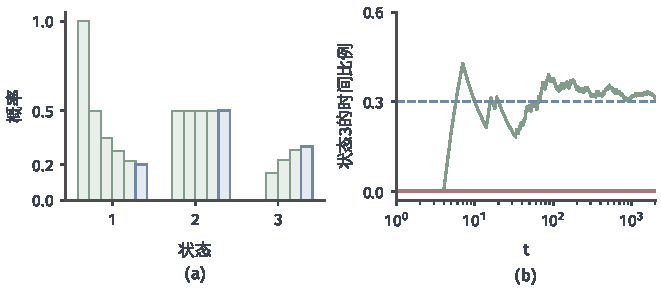
\includegraphics[width=112mm]{figures/07-probability/08-sampling-and-integration/matplotlib/sgen-chain-evolution/figure.pdf}
  \caption{三状态转移矩阵$\bm{K}$的分布传播与时间平均。(a)从状态$1$出发，每组左起五根绿色柱依次是$t=0,1,2,3,5$时的$\mu_t$，最右的蓝色柱是不变分布$\pi=(0.2,0.5,0.3)$；(b)一条模拟路径（种子$6$，横轴为对数刻度）上停在状态$3$的时间比例，绿线是$\bm{K}$，红线是“永远停在原地”的转移，蓝色虚线是$\pi(\{3\})=0.3$。}
  \label{fig:sgen-chain-evolution}
\end{BookInlineFigure}

\paragraph{不变不等于能到达}
不变性只说“从目标出发会留在目标”，不说“从别处出发会走到目标”。最极端的例子是始终停在原地的转移$K(x,\cdot)=\delta_x$，即单位矩阵。对它而言，任何分布都满足式~\eqref{eq:sgen-invariance}，目标分布当然也是不变分布。但从状态$1$出发，链永远停在$1$，停在状态$3$的时间比例恒为$0$，与$\pi(\{3\})=0.3$毫无关系，这就是图~\ref{fig:sgen-chain-evolution}(b)中的红线。

不那么极端的失败也很常见。若转移矩阵是分块对角的，例如状态$\{1,2\}$与$\{3\}$之间互不往来，从块$\{1,2\}$出发就永远看不到状态$3$。若转移在两个状态之间交替，$\bm{K}=\begin{bmatrix}0&1\\1&0\end{bmatrix}$，那么$(1/2,1/2)$是不变分布，从状态$1$出发的分布却在$(1,0)$与$(0,1)$之间来回摆动，永远不收敛，尽管时间比例趋于$1/2$。

所以MCMC的正确性分成两层。第一层是不变性，它是转移核的一个代数性质，下面三种更新都给出完整证明。第二层是从任意初值出发，分布收敛到$\pi$、时间平均收敛到目标期望，这需要状态之间能够互相到达（不可约）、链不陷入周期摆动（非周期）等条件。有限状态时，在不可约与非周期之下这两个结论都成立；一般状态空间需要更细的条件。这些长期性质的条件与证明可参考\BookChapterRef{chap:discrete-time-stochastic-processes}{卷九第3章“离散时间随机过程”}，也可查阅~\scite{math-meyn2009markov}。本章只证明不变性，并对每种更新指出它可能在哪里不能走遍目标。

\subsection{Metropolis--Hastings采样}
\label{sec:sgen-mh}

怎样构造一个以给定$\pi=\widetilde{p}/Z$为不变分布的转移？手里通常有一个容易抽样的局部建议，例如“在当前点附近随机迈一步”。这个建议本身一般不保持$\pi$，Metropolis--Hastings的做法是在建议之后加一道接受判定，把它修正成保持$\pi$的转移\scite{pgm-history-metropolis1953}\scite{pgm-history-hastings1970}。

\paragraph{主要思想：平衡每一对方向的概率流}
把$\pi$想象成状态之间的质量分配，转移一步就是把每个状态上的质量按转移概率分给各个状态。从$x$流向$y$的质量是$\pi(x)K(x,y)$，称为概率流。若每一对状态之间两个方向的流量相等，
\begin{equation}
  \pi(x)K(x,y)=\pi(y)K(y,x),
  \label{eq:sgen-detailed-balance-discrete}
\end{equation}
那么每个状态流出多少就流入多少，分布保持不变。这个条件称为\term{细致平衡}（detailed balance）。一般状态空间上，细致平衡写成对一切可测集$A,B$，
\begin{equation}
  \int_{A}K(x,B)\,\pi(\mathrm{d}x)=\int_{B}K(y,A)\,\pi(\mathrm{d}y),
  \label{eq:sgen-detailed-balance}
\end{equation}
即“从$A$流进$B$”等于“从$B$流进$A$”。

\begin{lemma}[细致平衡蕴含不变性]
\label{lem:sgen-detailed-balance}
若$\pi$与$K$满足式~\eqref{eq:sgen-detailed-balance}，则$\pi$是$K$的不变分布。
\end{lemma}

\begin{proof}
在式~\eqref{eq:sgen-detailed-balance}中取$A$为整个状态空间。左边是$\int K(x,B)\,\pi(\mathrm{d}x)$；右边中$K(y,\cdot)$是概率分布，$K(y,A)=1$，所以右边等于$\pi(B)$。这正是式~\eqref{eq:sgen-invariance}。
\end{proof}

细致平衡是充分条件而不是必要条件：沿圆周单向转圈的转移保持均匀分布不变，却在每一对方向上只有单向流量。它的好处是只需逐对检查，不必求和或积分，所以是构造转移最方便的工具。

现在设建议在状态$x$处的密度为$q(y\mid x)$（离散时是概率，连续时是关于Lebesgue测度的密度）。只用建议时，从$x$到$y$的流量正比于$\widetilde{p}(x)q(y\mid x)$，反向流量正比于$\widetilde{p}(y)q(x\mid y)$，二者一般不等。办法是把较大的一边按比例削减到较小的一边：从$x$到$y$的建议以概率$a(x,y)$接受，使
\[
  \widetilde{p}(x)q(y\mid x)a(x,y)=\min\bigl\{\widetilde{p}(x)q(y\mid x),\ \widetilde{p}(y)q(x\mid y)\bigr\}.
\]
右边关于$x,y$对称，流量自然平衡。解出$a$，得到
\begin{equation}
  a(x,y)=\min\Bigl\{1,\ \frac{\widetilde{p}(y)\,q(x\mid y)}{\widetilde{p}(x)\,q(y\mid x)}\Bigr\}.
  \label{eq:sgen-mh-acceptance}
\end{equation}
较小的一边接受概率为$1$，较大的一边按比值削减；被拒绝时留在原地。比值中$\widetilde{p}$出现在分子和分母，归一化常数$Z$约掉了，算法从头到尾不需要$Z$。

比值的定义需要交代。设当前状态$x$满足$\widetilde{p}(x)>0$，候选$y$由$q(\cdot\mid x)$产生，于是$q(y\mid x)>0$（概率为一），分母为正。若$\widetilde{p}(y)=0$或$q(x\mid y)=0$，比值为$0$，候选必被拒绝，所以链从$\{\widetilde{p}>0\}$出发就永远留在其中。

\begin{definition}[Metropolis--Hastings转移]
\label{def:sgen-mh}
设$\widetilde{p}\ge0$，$0<Z<\infty$，$S=\{x:\widetilde{p}(x)>0\}$。对$x\in S$，从$q(\cdot\mid x)$抽候选$y$，以式~\eqref{eq:sgen-mh-acceptance}的概率$a(x,y)$接受（令$X^{(t+1)}=y$），否则令$X^{(t+1)}=x$。对应的转移核为
\begin{equation}
  K(x,B)=\int_{B}q(y\mid x)\,a(x,y)\,\lambda(\mathrm{d}y)+r(x)\,\mathbf{1}_{B}(x),
  \label{eq:sgen-mh-kernel}
\end{equation}
其中$\lambda$是参考测度（计数测度或Lebesgue测度），
\begin{equation}
  r(x)=1-\int q(y\mid x)\,a(x,y)\,\lambda(\mathrm{d}y)
  \label{eq:sgen-mh-reject}
\end{equation}
是被拒绝而留在原地的概率。这种转移称为\term{Metropolis--Hastings算法}（Metropolis--Hastings algorithm）。
\end{definition}

\begin{theorem}[Metropolis--Hastings转移保持目标]
\label{thm:sgen-mh}
在定义~\ref{def:sgen-mh}的条件下，$\pi=\widetilde{p}/Z$与$K$满足细致平衡，因而$\pi$是$K$的不变分布。
\end{theorem}

\begin{proof}
对$\lambda$下的密度$\pi(x)=\widetilde{p}(x)/Z$，令
\[
  m(x,y)=\pi(x)\,q(y\mid x)\,a(x,y).
\]
先证
\[
  m(x,y)=\frac1Z\min\bigl\{\widetilde{p}(x)q(y\mid x),\ \widetilde{p}(y)q(x\mid y)\bigr\}.
\]
若$\widetilde{p}(x)q(y\mid x)>0$，把式~\eqref{eq:sgen-mh-acceptance}代入，乘开即得。若$\widetilde{p}(x)q(y\mid x)=0$，左边为零，右边的最小值也为零。所以$m(x,y)=m(y,x)$。

对可测集$A,B$，由式~\eqref{eq:sgen-mh-kernel}，
\[
  \int_{A}K(x,B)\,\pi(\mathrm{d}x)=\int_{A}\int_{B}m(x,y)\,\lambda(\mathrm{d}y)\,\lambda(\mathrm{d}x)+\int_{A\cap B}r(x)\,\pi(\mathrm{d}x).
\]
被积函数非负，可以交换积分次序；再用$m$的对称性，第一项对$A$与$B$对称。第二项是$r\pi$在$A\cap B$上的积分，本身对$A$与$B$对称。于是式~\eqref{eq:sgen-detailed-balance}成立，由引理~\ref{lem:sgen-detailed-balance}，$\pi$是不变分布。
\end{proof}

证明只用到两件事：接受概率使双向流量对称，被拒绝的质量留在原地。建议分布可以是任何能抽样、能计算密度的分布，这是Metropolis--Hastings的灵活之处。

\paragraph{为什么需要建议比}
若建议对称，$q(y\mid x)=q(x\mid y)$，式~\eqref{eq:sgen-mh-acceptance}简化为$\min\{1,\widetilde{p}(y)/\widetilde{p}(x)\}$，称为\term{Metropolis算法}（Metropolis algorithm）。模拟退火中的接受规则$\min\{1,\exp(-(f(y)-f(x))/T)\}$就是取$\widetilde{p}=\exp(-f/T)$的Metropolis规则。建议不对称时若仍用这个简化的比值，不变分布就会偏离目标，下面的三状态例子会算出偏离的结果。$q(x\mid y)/q(y\mid x)$这一项就是对建议偏向的修正：建议更爱往$y$走，就相应减少往$y$走的接受。

\paragraph{计算过程}
用$\{1,2,3\}$上的目标$\widetilde{p}=(2,5,3)$演示，$Z=10$对算法未知，$\pi=(0.2,0.5,0.3)$。建议在一条链上移动：从$1$总是建议$2$，从$3$总是建议$2$，从$2$以各$1/2$的概率建议$1$或$3$。建议不对称，例如$q(2\mid1)=1$而$q(1\mid2)=1/2$。

\needspace{6\baselineskip}
\paragraph{变量}
\begin{itemize}
  \item $x$：当前状态；$y$：候选状态。
  \item $a$：本步的接受概率，由式~\eqref{eq:sgen-mh-acceptance}计算。
  \item $u_{\mathrm{q}}$、$u_{\mathrm{a}}$：每步的两个基础随机数，前者用于抽候选（只在状态$2$需要），后者用于接受判定。
\end{itemize}

\paragraph{初始化}
取$x^{(0)}\in S$。例中$x^{(0)}=1$。四种可能的移动对应的接受概率可以预先算好：
\[
  \begin{aligned}
    a(1,2)&=\min\Bigl\{1,\frac{5\times\frac12}{2\times1}\Bigr\}=1,&\qquad
    a(2,1)&=\min\Bigl\{1,\frac{2\times1}{5\times\frac12}\Bigr\}=0.8,\\
    a(2,3)&=\min\Bigl\{1,\frac{3\times1}{5\times\frac12}\Bigr\}=1,&\qquad
    a(3,2)&=\min\Bigl\{1,\frac{5\times\frac12}{3\times1}\Bigr\}=\frac56.
  \end{aligned}
\]

\needspace{6\baselineskip}
\paragraph{每轮更新}
在第$t+1$步：
\begin{enumerate}
  \item \textbf{抽候选。}从$q(\cdot\mid x^{(t)})$抽$y$。例中状态$2$处，$u_{\mathrm{q}}\le0.5$时建议$1$，否则建议$3$；第一步$x^{(0)}=1$，候选$y=2$。

  \item \textbf{计算接受概率。}按式~\eqref{eq:sgen-mh-acceptance}计算$a(x^{(t)},y)$。例中第一步$a(1,2)=1$。

  \item \textbf{判定。}若$u_{\mathrm{a}}\le a$，令$x^{(t+1)}=y$；否则$x^{(t+1)}=x^{(t)}$。例中第一步$u_{\mathrm{a}}=0.37\le1$，接受，$x^{(1)}=2$。

  后四步使用的随机数与结果如下（空格表示该步不需要$u_{\mathrm{q}}$）：
  \begin{center}
    \small
    \begin{tabular}{@{}ccccccc@{}}
      \toprule
      $t$ & $x^{(t-1)}$ & $u_{\mathrm{q}}$ & $y$ & $a$ & $u_{\mathrm{a}}$ & $x^{(t)}$\\
      \midrule
      $2$ & $2$ & $0.62$ & $3$ & $1$ & $0.90$ & $3$（接受）\\
      $3$ & $3$ & & $2$ & $5/6$ & $0.88$ & $3$（拒绝）\\
      $4$ & $3$ & & $2$ & $5/6$ & $0.41$ & $2$（接受）\\
      $5$ & $2$ & $0.20$ & $1$ & $0.8$ & $0.85$ & $2$（拒绝）\\
      \bottomrule
    \end{tabular}
  \end{center}

  \item \textbf{停止。}做满预定的步数后停止。链本身没有自然的终点，步数要按下一章的误差分析决定。
\end{enumerate}
最终得到状态序列$1,2,3,3,2,2$。被拒绝的两步都把当前状态重复记录了一次，这些重复是转移的一部分，必须保留：删掉它们，状态$3$与状态$2$被访问的频率就会改变。

把接受概率乘上建议概率，得到转移矩阵
\[
  \bm{K}=\begin{bmatrix}0&1&0\\0.4&0.1&0.5\\0&\frac56&\frac16\end{bmatrix},
\]
其中$K(2,2)=1-0.4-0.5=0.1$与$K(3,3)=1/6$来自拒绝。逐对验证细致平衡：
\[
  \pi(1)K(1,2)=0.2=\pi(2)K(2,1),\qquad \pi(2)K(2,3)=0.25=\pi(3)K(3,2).
\]
图~\ref{fig:sgen-mh-three-state}画出建议与修正后的转移。

\begin{BookInlineFigure}
  \centering
  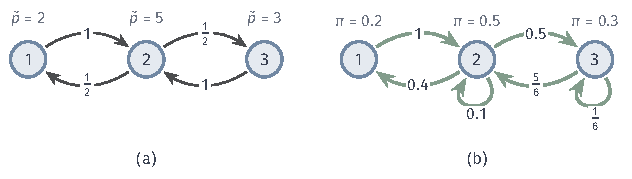
\includegraphics[width=107mm]{figures/07-probability/08-sampling-and-integration/tikz/sgen-mh-three-state/figure.pdf}
  \caption{三状态目标$\widetilde{p}=(2,5,3)$上的Metropolis--Hastings。(a)建议$q$：从端点总是走向中间，从中间各以$1/2$走向两端；(b)修正后的转移核，绿色箭头上是转移概率，自环来自拒绝。两个方向的概率流相等：$1\leftrightarrow2$都是$0.2$，$2\leftrightarrow3$都是$0.25$。}
  \label{fig:sgen-mh-three-state}
\end{BookInlineFigure}

若省去建议比，只用$\min\{1,\widetilde{p}(y)/\widetilde{p}(x)\}$，则$a(2,1)=0.4$、$a(2,3)=0.6$、$a(1,2)=a(3,2)=1$，转移矩阵的第二行变为$(0.2,0.5,0.3)$，第一、三行都是$(0,1,0)$。解$\pi\bm{K}=\pi$，由第一列得$\pi(1)=0.2\pi(2)$，由第三列得$\pi(3)=0.3\pi(2)$，归一化后
\[
  \pi=\Bigl(\frac{2}{15},\ \frac{2}{3},\ \frac{1}{5}\Bigr)\ne(0.2,\ 0.5,\ 0.3).
\]
中间状态被建议得多，又没有被修正，于是被过度访问。

\paragraph{随机游走建议}
连续状态最常用的建议是在当前点加一个对称扰动，$y=x+s\,\varepsilon$，$\varepsilon\sim\mathcal{N}(0,1)$，称为\term{随机游走Metropolis算法}（random-walk Metropolis algorithm）。步长$s$决定了接受率与移动距离之间的取舍。图~\ref{fig:sgen-rwmh-traces}在全章的混合目标上从$x=-2$出发各运行$3000$步：$s=0.3$时接受率约$0.83$，每步移动很小，链在左峰停留了很久，只有约$8\%$的时间在右边（目标是$70\%$）；$s=30$时几乎每个候选都落在目标概率很小的远处，接受率约$0.064$，链大段时间原地不动；$s=2.5$时接受率约$0.47$，两峰之间往来频繁。

\begin{BookInlineFigure}
  \centering
  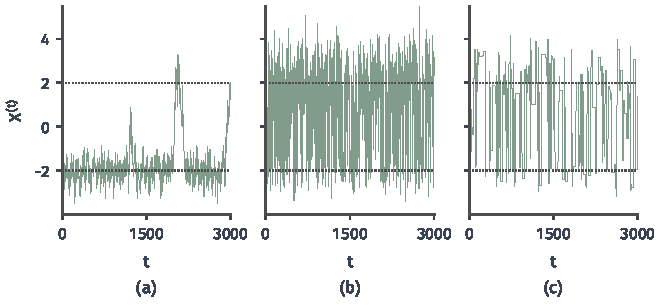
\includegraphics[width=112mm]{figures/07-probability/08-sampling-and-integration/matplotlib/sgen-rwmh-traces/figure.pdf}
  \caption{随机游走Metropolis在混合目标$0.3\,\mathcal{N}(-2,0.5^{2})+0.7\,\mathcal{N}(2,1)$上的轨迹，从$x=-2$出发，各$3000$步（种子$9$），虚线标出两个峰的位置。(a)$s=0.3$，接受率$0.83$；(b)$s=2.5$，接受率$0.47$；(c)$s=30$，接受率$0.064$，水平段是连续的拒绝。}
  \label{fig:sgen-rwmh-traces}
\end{BookInlineFigure}

三条链的转移都以同一个混合分布为不变分布，定理~\ref{thm:sgen-mh}对它们一视同仁。它们的差别全在“多快走遍目标”上，这是不变性之外的性质。每一步的成本是一次建议抽样、一次$\widetilde{p}$求值（当前点的值可以保存）和一个基础随机数。高维或尾部很重时，$\widetilde{p}$可能下溢为$0$或上溢，实际计算一律比较$\ln u_{\mathrm{a}}$与$\ln\widetilde{p}(y)-\ln\widetilde{p}(x)$加上建议比的对数。

\paragraph{建议必须能连通目标的支持}
不变性对任何建议都成立，包括那些根本到不了目标某些部分的建议。设目标是$[0,1]\cup[3,4]$上的均匀分布，建议是$y\sim\operatorname{Unif}(x-h,x+h)$。取$h=0.5$，从$x\in[0,1]$出发，候选落在$[x-0.5,x+0.5]\subset[-0.5,1.5]$中，凡是落在$[0,1]$之外的都有$\widetilde{p}(y)=0$而被拒绝，所以链永远留在$[0,1]$里。目标有一半质量在$[3,4]$上，链却一次也看不到。取$h=2.5$，候选可以越过长为$2$的空隙，链在两段之间往来（图~\ref{fig:sgen-mh-gap}）。

\begin{BookInlineFigure}
  \centering
  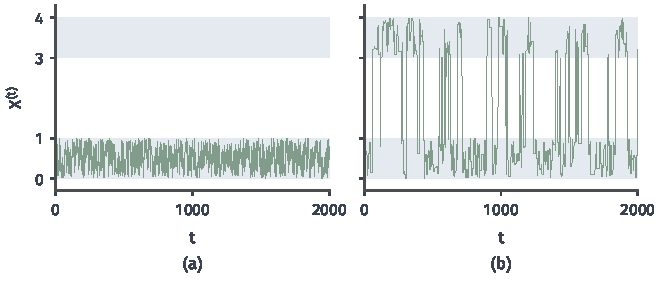
\includegraphics[width=112mm]{figures/07-probability/08-sampling-and-integration/matplotlib/sgen-mh-gap/figure.pdf}
  \caption{目标为$[0,1]\cup[3,4]$上的均匀分布（浅蓝带），建议为$\operatorname{Unif}(x-h,x+h)$，从$x=0.5$出发$2000$步（种子$10$）。(a)$h=0.5$：候选无法越过空隙，链停在$[0,1]$中，在$[3,4]$中的时间比例为$0$；(b)$h=2.5$：链在两段间往来，$[3,4]$中的时间比例为$0.39$，目标值为$0.5$。}
  \label{fig:sgen-mh-gap}
\end{BookInlineFigure}

这个例子中的失败在轨迹上一目了然，因为事先知道目标有两段。若不知道目标的形状，(a)的轨迹看起来是一条“混合良好”的链，在$[0,1]$上来回游走、接受率高达$0.75$，没有任何内部迹象提示还有一半质量没有访问。所以选择建议时，要从目标的结构出发论证它能连通支持，不能用接受公式的正确性或轨迹的外观代替这一论证。

\paragraph{独立建议}
另一种常用的建议是与当前状态无关的$q(y\mid x)=q(y)$，称为独立建议。记$w(x)=\widetilde{p}(x)/q(x)$，式~\eqref{eq:sgen-mh-acceptance}化为$\min\{1,w(y)/w(x)\}$：候选的权重比当前状态大就一定接受。它与拒绝采样用的是同一个比值，但不需要包络常数；代价是输出相关，而且若$q$在某处比目标轻得多，链一旦走到那里，$w(x)$很大，就会长时间被拒绝而停留。

\subsection{Gibbs采样}
\label{sec:sgen-gibbs}

多维目标的另一种局部信息是条件分布。设状态是$\bm{x}=(x_1,\dots,x_d)$，记$\bm{x}_{-i}$为去掉第$i$个坐标后的其余坐标。许多目标的联合分布难以直接抽样，但固定其余坐标后，第$i$个坐标的条件分布$\pi(\cdot\mid\bm{x}_{-i})$是一个熟悉的一维分布。这些条件分布称为完全条件分布。

\paragraph{单坐标更新}
保留其余坐标，只按完全条件分布重新抽第$i$个坐标，这一步的转移核记作$K_i$：从$\bm{x}$出发，新状态的第$i$个坐标服从$\pi(\cdot\mid\bm{x}_{-i})$，其余坐标与$\bm{x}$相同。轮流或随机地施行这些更新，就是\term{Gibbs采样}（Gibbs sampling）。

\begin{theorem}[单坐标更新保持目标]
\label{thm:sgen-gibbs}
设$\pi$是乘积空间上的分布，$\pi(\cdot\mid\bm{x}_{-i})$是给定其余坐标时第$i$个坐标的正则条件分布。则$\pi K_i=\pi$。
\end{theorem}

\begin{proof}
设$\bm{X}\sim\pi$，按$K_i$更新得到$\bm{X}'$，即$\bm{X}'_{-i}=\bm{X}_{-i}$，而给定$\bm{X}$时$X'_i$服从$\pi(\cdot\mid\bm{X}_{-i})$。新坐标只依赖$\bm{X}_{-i}$，旧的$X_i$在更新中被丢弃。于是$\bm{X}'_{-i}$的分布是$\pi$的边缘分布$\pi_{-i}$，给定$\bm{X}'_{-i}$时$X'_i$的条件分布是$\pi(\cdot\mid\bm{X}'_{-i})$。由第~\ref{chap:conditional-distributions}章，边缘分布与条件分布这一对确定了联合分布，它们恰好是$\pi$的边缘分布与条件分布，所以$\bm{X}'\sim\pi$。
\end{proof}

证明的直观是：更新前把$X_i$忘掉，剩下的$\bm{X}_{-i}$仍服从目标的边缘分布；再按正确的条件分布把$X_i$补回来，联合分布就复原了。也可以把单坐标更新看作建议为$q(\bm{y}\mid\bm{x})=\pi(y_i\mid\bm{x}_{-i})$的Metropolis--Hastings：此时$\bm{y}_{-i}=\bm{x}_{-i}$，比值
\[
  \frac{\pi(\bm{y})\,\pi(x_i\mid\bm{x}_{-i})}{\pi(\bm{x})\,\pi(y_i\mid\bm{x}_{-i})}=\frac{\pi_{-i}(\bm{x}_{-i})\pi(y_i\mid\bm{x}_{-i})\,\pi(x_i\mid\bm{x}_{-i})}{\pi_{-i}(\bm{x}_{-i})\pi(x_i\mid\bm{x}_{-i})\,\pi(y_i\mid\bm{x}_{-i})}=1,
\]
所以候选总被接受。

\paragraph{组合更新}
单坐标更新只动一个坐标，要让所有坐标都变化，需要把它们组合起来。按固定顺序依次施行$K_1,K_2,\dots,K_d$称为系统扫描，一轮的转移核是乘积$K_1K_2\cdots K_d$；每步以固定概率$c_i$随机选一个坐标更新，称为随机扫描，转移核是$\sum_ic_iK_i$，其中$c_i\ge0$、$\sum_ic_i=1$。两种组合都保持$\pi$：
\[
  \begin{gathered}
    \pi K_1K_2\cdots K_d=\pi K_2\cdots K_d=\dots=\pi,\\
    \pi\sum_ic_iK_i=\sum_ic_i\,\pi K_i=\sum_ic_i\pi=\pi.
  \end{gathered}
\]
随机扫描的条件是选择概率$c_i$固定，不能依赖当前状态。反例如下：设$\pi$是$\{0,1\}^{2}$上的均匀分布，规则为“$x_1=0$时更新第一个坐标，$x_1=1$时更新第二个坐标”。从$\pi$出发，$x_1=0$的一半质量更新$x_1$，其中一半变成$1$；$x_1=1$的一半质量只更新$x_2$，$x_1$保持为$1$。于是一步后
\[
  \mathbb{P}(X'_1=1)=\frac12\times\frac12+\frac12\times1=\frac34\ne\frac12 .
\]
每个$K_i$各自保持$\pi$，按状态挑选却把$x_1=1$的状态“锁住”了。

\paragraph{计算过程}
用二元高斯目标$\mathcal{N}(\bm{0},\bigl[\begin{smallmatrix}1&\rho\\\rho&1\end{smallmatrix}\bigr])$演示系统扫描，$\rho=0.8$。由第~\ref{chap:multivariate-distributions}章的高斯条件分布，两个完全条件分布是
\begin{equation}
  X_1\mid X_2=x_2\sim\mathcal{N}(\rho x_2,\,1-\rho^{2}),\qquad X_2\mid X_1=x_1\sim\mathcal{N}(\rho x_1,\,1-\rho^{2}).
  \label{eq:sgen-gibbs-gaussian}
\end{equation}

\needspace{6\baselineskip}
\paragraph{变量}
\begin{itemize}
  \item $(x_1,x_2)$：当前状态，每个坐标更新后立即覆盖。
  \item $z$：每次坐标更新使用的标准高斯数，由一个基础随机数经$\Phi^{-1}$得到。
\end{itemize}

\paragraph{初始化}
取一个初始状态。例中故意取在目标的边缘，$(x_1^{(0)},x_2^{(0)})=(2,2)$，以便看出链怎样走向中心。

\needspace{6\baselineskip}
\paragraph{每轮更新}
第$t+1$轮：
\begin{enumerate}
  \item \textbf{更新第一个坐标。}由式~\eqref{eq:sgen-gibbs-gaussian}，令
  \[
    x_1^{(t+1)}=\rho x_2^{(t)}+\sqrt{1-\rho^{2}}\,z .
  \]
  例中第一轮$z=\Phi^{-1}(0.37)\approx-0.3319$，
  \[
    x_1^{(1)}=0.8\times2+0.6\times(-0.3319)\approx1.4009 .
  \]

  \item \textbf{更新第二个坐标。}用刚得到的$x_1^{(t+1)}$，令
  \[
    x_2^{(t+1)}=\rho x_1^{(t+1)}+\sqrt{1-\rho^{2}}\,z' .
  \]
  例中第一轮$z'=\Phi^{-1}(0.80)\approx0.8416$，
  \[
    x_2^{(1)}=0.8\times1.4009+0.6\times0.8416\approx1.6257 .
  \]
  第二轮用$\Phi^{-1}(0.15)\approx-1.0364$与$\Phi^{-1}(0.62)\approx0.3055$，得到
  \[
    x_1^{(2)}\approx0.6787,\qquad x_2^{(2)}\approx0.7263 .
  \]

  \item \textbf{停止。}做满预定轮数后停止。
\end{enumerate}
最终得到状态序列$(2,2)$、$(1.4009,1.6257)$、$(0.6787,0.7263)$、\dots。每次只沿一个坐标轴移动，路径呈阶梯状。

\paragraph{相关性与移动速度}
相邻状态共用坐标，因而相关。在这个例子中可以算出相关的大小。把一轮的两步合起来，
\[
  X_1^{(t+1)}=\rho X_2^{(t)}+\sqrt{1-\rho^{2}}\,Z=\rho^{2}X_1^{(t)}+\rho\sqrt{1-\rho^{2}}\,Z''+\sqrt{1-\rho^{2}}\,Z,
\]
其中$Z''$是上一轮更新$X_2^{(t)}$所用的标准高斯数，$Z,Z''$与$X_1^{(t)}$独立。若链已处于目标分布，$\operatorname{Var}(X_1^{(t)})=1$，于是
\[
  \operatorname{Cov}\bigl(X_1^{(t+1)},X_1^{(t)}\bigr)=\rho^{2},
\]
逐轮迭代得到相隔$k$轮的相关系数为$\rho^{2k}$。$\rho=0.8$时每轮相关系数为$0.64$，几轮之后就基本忘记了起点；$\rho=0.99$时每轮为$0.98$，要约$35$轮相关系数才降到一半。

图~\ref{fig:sgen-gibbs-path}画出两种情形下前$20$轮的路径。目标沿对角线拉长时，每个完全条件分布都很窄，宽度为$\sqrt{1-\rho^{2}}$，链只能沿坐标轴迈小步，在狭长的山脊上缓慢挪动。这是Gibbs采样的典型弱点：坐标之间强相关时移动很慢，此时把强相关的坐标合成一块整体更新，或者换一套坐标，会有明显改善。

\begin{BookInlineFigure}
  \centering
  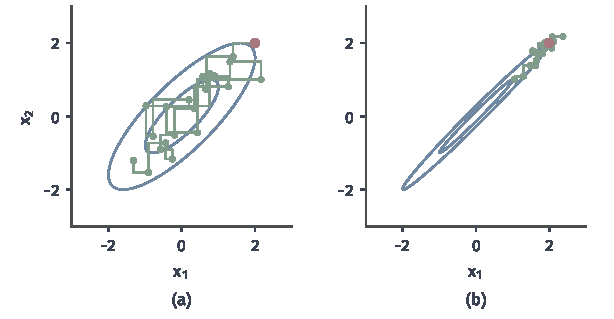
\includegraphics[width=104mm]{figures/07-probability/08-sampling-and-integration/matplotlib/sgen-gibbs-path/figure.pdf}
  \caption{二元高斯目标上的系统扫描Gibbs采样，从红点$(2,2)$出发$20$轮，前两轮使用正文中的随机数，其后的标准高斯数取自种子$12$。蓝色椭圆是目标的$1$倍与$2$倍等概率线，绿色阶梯是路径，绿点是每轮结束时的状态。(a)$\rho=0.8$，链很快进入中心并四处移动；(b)$\rho=0.99$，同样的随机数下链只沿山脊挪动了一小段。}
  \label{fig:sgen-gibbs-path}
\end{BookInlineFigure}

\paragraph{条件更新可能走不通}
Gibbs采样只沿坐标轴移动，目标的支持形状可能挡住去路。设目标是$[0,1]^{2}\cup[2,3]^{2}$上的均匀分布。当$x_2\in[0,1]$时，$x_1$的完全条件分布是$[0,1]$上的均匀分布，因为水平线$\{x_2=\text{常数}\}$只与下面的正方形相交；同理$x_1\in[0,1]$时$x_2$也只能在$[0,1]$中取值。从下面的正方形出发，链永远留在那里，尽管每一步都正确地保持了目标。若把两个正方形改成相互重叠的$[0,2]^{2}\cup[1,3]^{2}$，穿过重叠带的水平线同时碰到两个正方形，链就可以过去（图~\ref{fig:sgen-gibbs-reducible}）。

\begin{BookInlineFigure}
  \centering
  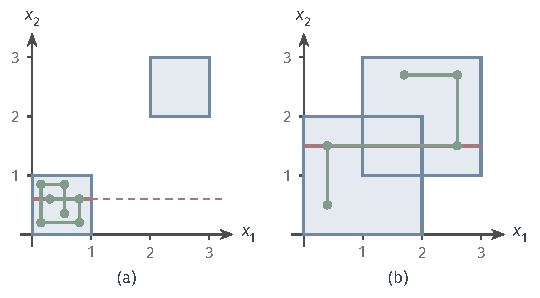
\includegraphics[width=91mm]{figures/07-probability/08-sampling-and-integration/tikz/sgen-gibbs-reducible/figure.pdf}
  \caption{支持形状对Gibbs采样的影响，目标是浅蓝区域上的均匀分布。(a)两个正方形在两个坐标方向上都不重叠，红色实线是$x_2=0.6$时$x_1$的条件分布所在区间，延长的红色虚线碰不到另一个正方形，绿色路径永远留在下方；(b)两个正方形部分重叠，红线$x_2=1.5$同时穿过两者，绿色路径经由它进入上方的正方形。}
  \label{fig:sgen-gibbs-reducible}
\end{BookInlineFigure}

每轮Gibbs采样的成本是$d$次条件抽样。完全条件分布是标准分布时，每次只需常数个基础随机数；不是标准分布时，每次条件抽样可能要用逆变换的数值反演、拒绝采样，甚至在这一坐标上做一步Metropolis--Hastings。后一种做法仍保持$\pi$，因为它是一个以$\pi(\cdot\mid\bm{x}_{-i})$为不变分布的一维更新，套上定理~\ref{thm:sgen-gibbs}的证明即可。

\subsection{Hamilton采样}
\label{sec:sgen-hmc}

随机游走建议和坐标更新都只能迈小步：步子大了接受率就低，坐标强相关时又只能沿轴挪动。若目标在欧氏空间上有光滑的正密度，梯度给出了“往哪里走概率不会掉太多”的信息。Hamilton采样借用力学中的运动方程，沿着保持总能量的轨道一次走出很远，再用接受判定修正数值误差\scite{pgm-sampling-neal2011}。

\paragraph{辅助动量与Hamilton量}
设目标为$\pi(\bm{x})\propto\exp(-U(\bm{x}))$，$\bm{x}\in\mathbb{R}^{d}$，其中$U=-\ln\widetilde{p}$二阶连续可微，称为势能。引入与$\bm{x}$同维、相互独立的辅助变量$\bm{p}\sim\mathcal{N}(\bm{0},\bm{I})$，称为动量。$(\bm{x},\bm{p})$的联合密度正比于
\begin{equation}
  \exp\bigl(-H(\bm{x},\bm{p})\bigr),\qquad H(\bm{x},\bm{p})=U(\bm{x})+\tfrac12\lVert\bm{p}\rVert_2^{2},
  \label{eq:sgen-hamiltonian}
\end{equation}
$H$称为Hamilton量，第二项是动能。联合密度分解为$\bm{x}$的因子与$\bm{p}$的因子之积，所以$\bm{x}$的边缘分布就是$\pi$：只要构造出保持联合分布的链，丢掉动量即可。

在相空间中沿Hamilton方程
\[
  \frac{\mathrm{d}\bm{x}}{\mathrm{d}t}=\bm{p},\qquad \frac{\mathrm{d}\bm{p}}{\mathrm{d}t}=-\nabla U(\bm{x})
\]
运动，有两条关键性质：$H$沿轨道守恒，相空间体积在流映射下保持不变，可参考\BookChapterRef{chap:ode-sensitivity}{卷六第4章“解的敏感性”}。$H$守恒意味着联合密度沿轨道不变，体积保持意味着把一块区域搬走时不需要Jacobian修正。轨道可以穿过目标的大片区域，同时停留在同一个密度水平上，这正是随机游走做不到的。

\paragraph{确定性提议的接受判定}
精确的Hamilton流一般解不出来，要用数值格式近似。先说明：任何满足两个条件的确定性映射，都可以配上一道接受判定而精确保持目标。

\begin{lemma}[对合映射的Metropolis修正]
\label{lem:sgen-involution}
设$\rho$是$\mathbb{R}^{m}$上的概率密度，$\Phi:\mathbb{R}^{m}\to\mathbb{R}^{m}$满足$\Phi\circ\Phi=\mathrm{id}$（对合），且保持体积（$\lvert\det D\Phi\rvert\equiv1$）。从$\bm{z}$出发，提议$\Phi(\bm{z})$，以概率$\min\{1,\rho(\Phi(\bm{z}))/\rho(\bm{z})\}$接受，否则留在$\bm{z}$。则$\rho$满足细致平衡，因而是不变分布。
\end{lemma}

\begin{proof}
从$\bm{z}$出发、被接受的移动所带的概率流密度为
\[
  m(\bm{z})=\rho(\bm{z})\min\Bigl\{1,\frac{\rho(\Phi(\bm{z}))}{\rho(\bm{z})}\Bigr\}=\min\bigl\{\rho(\bm{z}),\rho(\Phi(\bm{z}))\bigr\},
\]
$\rho(\bm{z})=0$时两边都取$0$。由$\Phi\circ\Phi=\mathrm{id}$，把$\bm{z}$换成$\Phi(\bm{z})$只是交换最小值中的两项，所以
\[
  m(\Phi(\bm{z}))=m(\bm{z}).
\]对可测集$A,B$，从$A$经接受的移动进入$B$的流量为
\[
  \int\mathbf{1}_{A}(\bm{z})\,\mathbf{1}_{B}(\Phi(\bm{z}))\,m(\bm{z})\,\mathrm{d}\bm{z}.
\]
作换元$\bm{z}=\Phi(\bm{w})$。由体积保持，体积元不变；由对合，$\Phi(\bm{z})=\bm{w}$；再由$m$在$\Phi$下不变，上式化为
\[
  \int\mathbf{1}_{A}(\Phi(\bm{w}))\,\mathbf{1}_{B}(\bm{w})\,m(\bm{w})\,\mathrm{d}\bm{w},
\]
这正是从$B$经接受的移动进入$A$的流量。被拒绝时留在原地，这部分流量对$A,B$对称。所以式~\eqref{eq:sgen-detailed-balance}成立，由引理~\ref{lem:sgen-detailed-balance}，$\rho$是不变分布。
\end{proof}

两个条件各有作用。对合使提议“可以原路返回”：从$\bm{z}$提议$\Phi(\bm{z})$，从$\Phi(\bm{z})$恰好提议回$\bm{z}$，正反两个方向成对出现。体积保持使换元时不出现Jacobian因子，接受概率只是密度之比。缺了体积保持，比值中还要乘上$\lvert\det D\Phi(\bm{z})\rvert$。

\paragraph{蛙跳格式}
求解Hamilton方程的\term{蛙跳格式}（leapfrog scheme）以步长$\varepsilon$做三个子步：
\begin{equation}
  \bm{p}_{1/2}=\bm{p}-\frac{\varepsilon}{2}\nabla U(\bm{x}),\qquad
  \bm{x}'=\bm{x}+\varepsilon\,\bm{p}_{1/2},\qquad
  \bm{p}'=\bm{p}_{1/2}-\frac{\varepsilon}{2}\nabla U(\bm{x}'),
  \label{eq:sgen-leapfrog}
\end{equation}
记这一步为$\Psi_{\varepsilon}:(\bm{x},\bm{p})\mapsto(\bm{x}',\bm{p}')$。

它保持体积：三个子步各自只改变一组变量，改变量只依赖另一组变量，例如第一步$(\bm{x},\bm{p})\mapsto(\bm{x},\bm{p}-\tfrac{\varepsilon}{2}\nabla U(\bm{x}))$的Jacobian矩阵是分块下三角的，对角块都是单位矩阵，行列式为$1$。三个这样的映射复合，行列式仍为$1$。

它在动量反转下可逆。记$F(\bm{x},\bm{p})=(\bm{x},-\bm{p})$。从$(\bm{x}',-\bm{p}')$再做一步$\Psi_{\varepsilon}$，三个子步依次给出
\[
  \begin{aligned}
    -\bm{p}'-\tfrac{\varepsilon}{2}\nabla U(\bm{x}')&=-\bm{p}_{1/2},\\
    \bm{x}'+\varepsilon(-\bm{p}_{1/2})&=\bm{x},\\
    -\bm{p}_{1/2}-\tfrac{\varepsilon}{2}\nabla U(\bm{x})&=-\bm{p},
  \end{aligned}
\]
第一行用到式~\eqref{eq:sgen-leapfrog}的第三式，第二、三行用到第二式和第一式。所以先走一步、反转、再走一步，得到的是$(\bm{x},-\bm{p})$，即$\Psi_{\varepsilon}F\Psi_{\varepsilon}=F$。由$F\circ F=\mathrm{id}$，这等价于$F\Psi_{\varepsilon}F=\Psi_{\varepsilon}^{-1}$。连做$L$步时，
\[
  F\Psi_{\varepsilon}^{L}F=(F\Psi_{\varepsilon}F)^{L}=\Psi_{\varepsilon}^{-L},
\]
所以$\Phi=F\circ\Psi_{\varepsilon}^{L}$满足$\Phi\circ\Phi=\mathrm{id}$，并且保持体积。精确的Hamilton流有同样两条性质，蛙跳格式在离散后仍完整保留了它们，失去的只是$H$的守恒。

\paragraph{完整的一步}
\term{Hamilton采样}（Hamiltonian Monte Carlo）的一步由两部分组成：
\begin{enumerate}
  \item \textbf{刷新动量。}丢弃旧的动量，重新抽$\bm{p}\sim\mathcal{N}(\bm{0},\bm{I})$。在联合分布下$\bm{p}$与$\bm{x}$独立，这一步就是对$\bm{p}$的一次Gibbs更新，由定理~\ref{thm:sgen-gibbs}，它保持联合分布。

  \item \textbf{轨道提议与修正。}从$(\bm{x},\bm{p})$出发做$L$步蛙跳，再反转动量，得到
  \[
    (\bm{x}^{*},\bm{p}^{*})=F\Psi_{\varepsilon}^{L}(\bm{x},\bm{p}),
  \]
  以概率
  \begin{equation}
    \min\Bigl\{1,\ \exp\bigl(H(\bm{x},\bm{p})-H(\bm{x}^{*},\bm{p}^{*})\bigr)\Bigr\}
    \label{eq:sgen-hmc-accept}
  \end{equation}
  接受$\bm{x}^{*}$，否则保留$\bm{x}$。由引理~\ref{lem:sgen-involution}（取$\rho\propto\mathrm{e}^{-H}$），这一步也保持联合分布。
\end{enumerate}
两步复合仍保持联合分布，于是$\bm{x}$的边缘分布$\pi$不变。式~\eqref{eq:sgen-hmc-accept}只用到$U$的值差，归一化常数照样约掉。

四个组成部分各司其职。刷新动量改变能量水平：若不刷新，链只在一条近似的能量等值面上移动，无法到达其他密度水平。蛙跳格式的可逆与保体积使接受概率只含能量差。动量反转把提议变成对合，满足引理的条件；下一步开始时动量会被重新抽取，而$\mathcal{N}(\bm{0},\bm{I})$关于$\bm{p}\mapsto-\bm{p}$对称，所以实际程序中常省去这一反转。接受判定修正离散化误差：精确流下$H$守恒，接受概率为$1$，蛙跳的能量误差越小，接受率越高。

\paragraph{计算过程}
用一维标准高斯目标演示，$U(x)=x^{2}/2$，$\nabla U(x)=x$，步长$\varepsilon=0.5$，每次提议走$L=2$步。

\needspace{6\baselineskip}
\paragraph{变量}
\begin{itemize}
  \item $x$：当前位置；$p$：本次刷新的动量。
  \item $(x_{\ell},p_{\ell})$：蛙跳第$\ell$步后的位置与动量，$\ell=0,\dots,L$。
  \item $\Delta H$：轨道终点与起点的能量差。
\end{itemize}

\paragraph{初始化}
给定当前位置。例中$x=1$。

\needspace{6\baselineskip}
\paragraph{每轮更新}
\begin{enumerate}
  \item \textbf{刷新动量。}抽$p\sim\mathcal{N}(0,1)$。例中由$u=0.80$得$p=\Phi^{-1}(0.80)\approx0.8416$，于是
  \[
    H(x_0,p_0)=\frac{1^{2}}{2}+\frac{0.8416^{2}}{2}\approx0.8542 .
  \]

  \item \textbf{蛙跳$L$步。}按式~\eqref{eq:sgen-leapfrog}迭代。例中第一步
  \[
    \begin{aligned}
      p_{1/2}&=0.8416-0.25\times1=0.5916,\\
      x_1&=1+0.5\times0.5916=1.2958,\\
      p_1&=0.5916-0.25\times1.2958\approx0.2677 .
    \end{aligned}
  \]
  第二步
  \[
    \begin{aligned}
      p_{3/2}&\approx0.2677-0.25\times1.2958=-0.0563,\\
      x_2&\approx1.2958+0.5\times(-0.0563)=1.2677,\\
      p_2&\approx-0.0563-0.25\times1.2677=-0.3732 .
    \end{aligned}
  \]

  \item \textbf{反转并计算能量差。}令$p^{*}=-p_2$，它不改变动能。例中
  \[
    H(x_2,p^{*})=\frac{1.2677^{2}}{2}+\frac{0.3732^{2}}{2}\approx0.8731,\qquad \Delta H\approx0.0190 .
  \]

  \item \textbf{判定。}由式~\eqref{eq:sgen-hmc-accept}，接受概率为$\min\{1,\mathrm{e}^{-\Delta H}\}$。例中$\mathrm{e}^{-0.0190}\approx0.9812$，取基础随机数$u=0.37$，接受，新位置为$1.2677$。
\end{enumerate}
最终一次迭代用到$x_0,x_1,x_2$三处的梯度（$x_1$处的梯度在两步之间重复使用）和两个基础随机数，位置从$1$移到$1.2677$。能量只变了约$0.019$，所以几乎必然接受。

\paragraph{步长与轨道长度}
步长决定能量误差。对这个一维例子，式~\eqref{eq:sgen-leapfrog}是线性映射，代入$\nabla U(x)=x$可得
\[
  \begin{bmatrix}x'\\p'\end{bmatrix}=
  \begin{bmatrix}1-\varepsilon^{2}/2&\varepsilon\\-\varepsilon(1-\varepsilon^{2}/4)&1-\varepsilon^{2}/2\end{bmatrix}
  \begin{bmatrix}x\\p\end{bmatrix}.
\]
矩阵的行列式为$1$，迹为$2-\varepsilon^{2}$。$0<\varepsilon<2$时迹的绝对值小于$2$，两个特征值是单位圆上的一对共轭复数，迭代点在一个椭圆上转动，能量误差有界；$\varepsilon>2$时有一个特征值的绝对值大于$1$，轨道按指数发散，接受率趋于零。若目标的标准差为$\sigma$，同样的计算给出稳定条件$\varepsilon<2\sigma$；多维时由最窄的方向决定。

图~\ref{fig:sgen-leapfrog}(a)画出$\varepsilon=0.5$与$\varepsilon=1.8$的轨道，前者紧贴精确的圆形轨道，后者被拉成扁椭圆。(b)是固定轨道总长约为$3$时，轨道上最大能量误差随$\varepsilon$的变化，在稳定范围内大致与$\varepsilon^{2}$成正比。对一般的光滑$U$，固定轨道长度时能量误差为$O(\varepsilon^{2})$，证明要用到数值积分的误差分析，这里只用图中的数值说明。

\begin{BookInlineFigure}
  \centering
  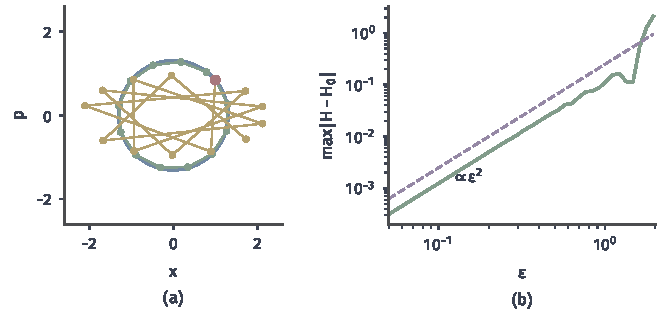
\includegraphics[width=112mm]{figures/07-probability/08-sampling-and-integration/matplotlib/sgen-leapfrog/figure.pdf}
  \caption{标准高斯目标的蛙跳格式，起点为红点$(x,p)=(1,\Phi^{-1}(0.8))$。(a)蓝线是精确的Hamilton轨道（能量等值线），绿色是$\varepsilon=0.5$的$12$步，黄色是$\varepsilon=1.8$的$12$步；(b)轨道总长约为$3$（$L=\operatorname{round}(3/\varepsilon)$）时轨道上的最大能量误差，紫色虚线是斜率为$2$的参考线。}
  \label{fig:sgen-leapfrog}
\end{BookInlineFigure}

轨道长度$L\varepsilon$决定一次能走多远。太短时与随机游走无异；太长时轨道可能绕回起点附近，例如标准高斯的精确轨道周期为$2\pi$，走满一周等于白走。每次提议的成本是$L$次梯度计算，比较方法时应在相同的梯度或密度计算次数下比较。图~\ref{fig:sgen-hmc-rw}在相关系数为$0.95$的二元高斯目标上做了这样的比较：$200$次密度计算的随机游走Metropolis（接受率$0.69$）还在山脊的一端徘徊，$200$次梯度计算的Hamilton采样（$20$次提议，每次$10$步，接受率$0.85$）已在整个椭圆上来回。

\begin{BookInlineFigure}
  \centering
  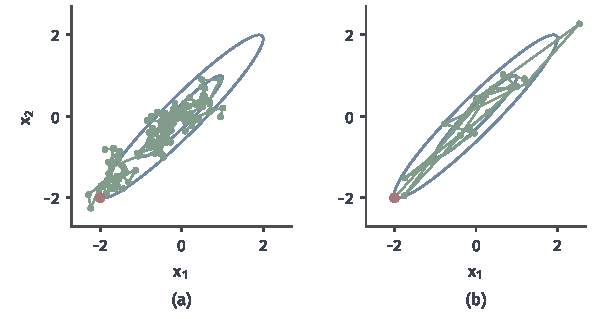
\includegraphics[width=104mm]{figures/07-probability/08-sampling-and-integration/matplotlib/sgen-hmc-rw/figure.pdf}
  \caption{相关系数$0.95$的二元高斯目标，从红点$(-2,-2)$出发，计算量相同。(a)随机游走Metropolis，步长$0.25$，$200$步；(b)Hamilton采样，$\varepsilon=0.18$、$L=10$，$20$次提议。两者都用种子$13$，蓝色椭圆是$1$倍与$2$倍等概率线。}
  \label{fig:sgen-hmc-rw}
\end{BookInlineFigure}

Hamilton采样的适用范围也由它的条件划定。它需要欧氏空间上光滑、处处为正的密度和可以计算的梯度，离散变量或有硬边界的支持都要另行处理。多峰目标中，两个峰之间的低密度区要靠刷新动量时偶尔得到的高能量才能越过，峰间隔得远时同样会长期困在一个峰中。

\section{生成结果的核验}
\label{sec:sgen-checks}

一个生成程序写好之后，怎样确认它给出的是想要的东西？前面几节其实已经区分了两类要核对的性质：直接生成要核对每个样本的分布及样本之间的独立性，链式更新要核对目标是否为不变分布以及链能否走遍目标。此外，实际程序与数学方法之间还隔着停止规则、有限精度和数值近似，它们各自会引入偏差。本节逐项说明怎样核对，以及经验检查能说明什么、不能说明什么。

\paragraph{直接生成：分布与独立性}
直接生成的正确性有完整的数学判据：输出分布满足式~\eqref{eq:sgen-correct-law}。前几节对每种方法都给出了这样的证明，核验时要逐条对照证明用到的条件是否在程序中成立，例如分位数是否对所有$u$有误差界、包络常数是否真正满足式~\eqref{eq:sgen-envelope}、混合采样的两步是否使用了不同的随机数。

独立性来自输入：每个样本只使用自己的一组基础随机数，组与组互不重叠。核对时要看程序是否在样本之间共用了状态，例如为了“节省”而把上一个样本剩余的随机数或中间结果留给下一个样本。只要输入不重叠，同分布且独立就有保证，样本个数再多也不会产生相关。

\paragraph{链式更新：不变性、可达性与相关性}
链的不变性同样可以证明，并且可以对小问题做精确的数值核对。把程序中的接受规则原样用在一个有限状态的小目标上（例如第~\ref{sec:sgen-mh}节的三状态目标），按程序逻辑写出完整的转移矩阵$\bm{K}$，直接计算$\pi\bm{K}-\pi$。它应在舍入误差以内为零。这种核对不依赖任何模拟，能发现遗漏建议比、遗漏拒绝时的重复记录之类的错误：前面已经算出，遗漏建议比会把不变分布变成$(2/15,2/3,1/5)$。

可达性无法用这种方式核对，它是关于整个目标支持的全局性质，要从目标的结构论证，例如说明建议分布能以正概率从任一点走到任一个正概率区域附近。第~\ref{sec:sgen-mh}节与第~\ref{sec:sgen-gibbs}节的两个反例都是每一步都正确、整体却走不通的情形。

即使链从目标分布出发，各个状态的边缘分布都是$\pi$，状态之间也一般相关，不能当作独立样本。图~\ref{fig:sgen-checks}(c)是二元高斯Gibbs采样中$X_1$的样本自相关，与第~\ref{sec:sgen-gibbs}节算出的$\rho^{2k}$一致：$\rho=0.99$时相隔$40$轮仍有约$0.5$的相关。相关性对积分误差的影响是下一章的内容，这里只需记住：链的输出不满足独立样本的假设。

\paragraph{停止规则带来的偏差}
理论上的方法常常假设可以无限地做下去，程序却必须停下来，停止的方式会改变输出分布。

拒绝采样理论上试到接受为止。若程序为了限制时间，最多试$T$次，全部失败时返回最后一个候选，输出就不再服从$\pi$。记接受率为$a$，前$n-1$次失败、第$n$次接受的概率是$(1-a)^{n-1}a$，接受的样本服从$\pi$；$T$次全部失败的概率是$(1-a)^{T}$，此时返回的候选服从“候选在被拒绝条件下”的分布。由定理~\ref{thm:sgen-rejection}的计算，候选被拒绝且落在$A$中的概率是$\int_{A}q-\tfrac1M\int_{A}\widetilde{p}$，记其条件分布为$R$。于是输出分布为
\begin{equation}
  \bigl(1-(1-a)^{T}\bigr)\,\pi+(1-a)^{T}R .
  \label{eq:sgen-capped-rejection}
\end{equation}
偏差的权重$(1-a)^{T}$随$T$几何下降，但永远不为零。以$\operatorname{Beta}(2,2)$的例子计算，$a=2/3$，$R$的密度为
\[
  \frac{1-4x(1-x)}{1/3}=3(1-2x)^{2}.
\]
$T=1$时式~\eqref{eq:sgen-capped-rejection}给出$\tfrac23\cdot6x(1-x)+\tfrac13\cdot3(1-2x)^{2}=1$，即输出就是建议分布本身，这与“只试一次就交出候选”的直觉一致（图~\ref{fig:sgen-capped-rejection}）。

\begin{BookInlineFigure}
  \centering
  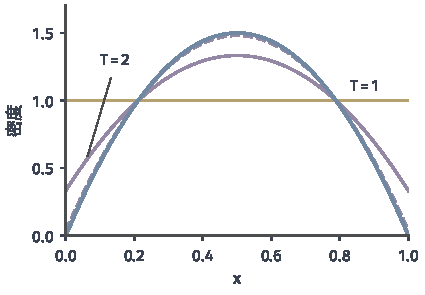
\includegraphics[width=72mm]{figures/07-probability/08-sampling-and-integration/matplotlib/sgen-capped-rejection/figure.pdf}
  \caption{最多试$T$次的拒绝采样的输出密度，目标$\operatorname{Beta}(2,2)$，建议$\operatorname{Unif}(0,1)$，$M=1/4$。黄线$T=1$（等于建议分布），紫色实线$T=2$，紫色虚线$T=4$，蓝线是目标$6x(1-x)$。偏差权重为$(1/3)^{T}$。}
  \label{fig:sgen-capped-rejection}
\end{BookInlineFigure}

链式更新也有同样的问题。从$\mu_0$出发运行$t$步，$X^{(t)}$的分布是$\mu_0K^{t}$，一般不等于$\pi$。第~\ref{sec:sgen-invariance}节的三状态例子从状态$1$出发，$5$步后的分布是$(0.219,0.5,0.281)$，离$\pi=(0.2,0.5,0.3)$还有可见的差距。“等到轨迹看起来稳定再开始记录”是一种依赖于已生成数据的停止规则，它本身也会改变被记录状态的分布。这些偏差有多大、怎样控制，是下一章讨论链初值影响时的主题。

\paragraph{有限精度与数值近似}
每一种数值近似都在数学方法与程序输出之间插入了一个误差，核验时要逐个列出。逆变换中的数值反演按引理~\ref{lem:sgen-inversion-error}改变输出的分布函数，误差界必须对全部$u$成立；协方差因子的舍入误差改变输出的协方差。链式更新中，接受比值若直接用密度相除，可能出现下溢后的$0/0$，应改用对数。Hamilton采样中步长超过稳定范围时轨道发散，表现为能量差变成很大的数或非数值，程序应把它作为拒绝处理并报告，而不是悄悄跳过这一步：跳过等于改变了转移核。

这些近似之外，还有基础随机数本身与理想模型的差距（第~\ref{sec:sgen-uniform}节）。近似生成造成的偏差不会随样本数增加而消失，它与样本数决定的随机波动是两种不同的误差，下一章将分开评价。

\paragraph{经验检查的作用与边界}
直方图、样本矩、自相关与轨迹图是最常用的经验检查。它们能发现问题，却不能证明正确。图~\ref{fig:sgen-checks}给出三种情形。

\begin{BookInlineFigure}
  \centering
  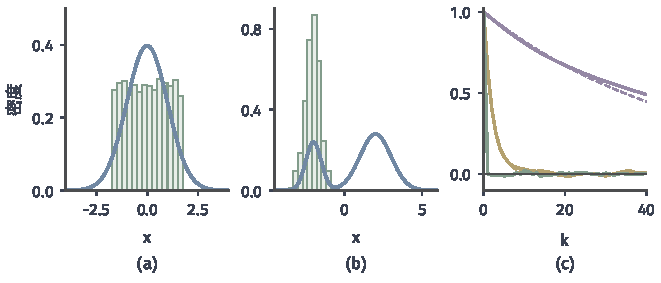
\includegraphics[width=112mm]{figures/07-probability/08-sampling-and-integration/matplotlib/sgen-checks/figure.pdf}
  \caption{经验检查能看出什么。(a)$\operatorname{Unif}(-\sqrt3,\sqrt3)$的$5000$个样本（种子$14$），样本均值$0.006$、方差$1.007$，与$\mathcal{N}(0,1)$（蓝线）的前两阶矩相同，直方图却明显不同；(b)第~\ref{sec:sgen-mh}节步长$0.3$的随机游走Metropolis的前$1000$个状态，直方图是一个干净的单峰，蓝线是混合目标；(c)二元高斯Gibbs采样中$X_1$的样本自相关（$20000$轮，种子$15$），黄线$\rho=0.8$，紫线$\rho=0.99$，虚线是$\rho^{2k}$，绿线是独立样本。}
  \label{fig:sgen-checks}
\end{BookInlineFigure}

(a)说明低阶矩相符不能说明分布正确：均匀分布$\operatorname{Unif}(-\sqrt3,\sqrt3)$的均值为$0$、方差为$1$，与标准高斯相同。若某个“高斯生成器”实际输出的是它，只检查均值与方差永远发现不了，直方图则一眼可见。反过来，直方图只比较到分箱的分辨率，比分箱更细的偏差（例如第~\ref{sec:sgen-transform}节固定轮数二分法造成的离散化）以及远处尾部的偏差，直方图也看不出来。

(b)说明经验检查只能看到已经访问过的区域。链的前$1000$个状态全部在左峰附近，直方图形状规则，与左峰的密度相符；单看这批状态，没有任何迹象提示右边还有一个占$70\%$质量的峰。只有事先知道目标有两个峰，才能看出问题。同理，从不同初值出发的多条链若都没有找到某个区域，它们彼此一致也不能说明那个区域不存在。

(c)说明自相关可以量出链的“记性”有多长，却不能说明链已经走遍了目标：一条困在单峰中的链，在峰内的自相关可能很快衰减。

所以经验检查的作用是排除明显的错误：它们发现的偏差是真实的，没有发现偏差则不构成证明。正确性的依据仍是前面各节的证明，加上对可达性的结构论证；经验检查在此基础上补充核对程序是否忠实地实现了证明中的方法。

\section{本章小结}
\label{sec:sgen-summary}

本章从独立均匀的基础随机数出发，回答了章首的问题：怎样把它们加工成给定分布的样本，以及加工结果是什么性质的样本。方法的选择取决于目标分布提供了哪些可以计算的信息。表~\ref{tab:sgen-methods}把各种方法放在一起比较。

\begin{BookInlineTable}
  \centering
  \small
  \begin{tabular}{@{}llll@{}}
    \toprule
    方法 & 需要的信息 & 输出 & 主要成本与失效 \\
    \midrule
    逆变换 & 分位数或可反演的$F$ & 独立样本 & 数值反演误差、尾部截断 \\
    仿射高斯 & 协方差因子 & 独立样本 & 一次分解，奇异时退化 \\
    分步生成 & 成分或条件分布 & 独立样本 & 各步须用不同随机数 \\
    拒绝采样 & $\widetilde{p}$、建议、包络$M$ & 独立样本 & 平均$M/Z$次试验 \\
    MH & $\widetilde{p}$、建议密度 & 相关的链 & 步长取舍、支持连通 \\
    Gibbs & 完全条件分布 & 相关的链 & 强相关时慢、支持形状 \\
    Hamilton & $\nabla U$、光滑正密度 & 相关的链 & 每步$L$次梯度、步长稳定 \\
    \bottomrule
  \end{tabular}
  \caption{采样生成方法的比较。前四种输出服从目标分布的独立样本；后三种输出以目标为不变分布的链，状态相关，能否走遍目标需另行论证。}
  \label{tab:sgen-methods}
\end{BookInlineTable}

直接生成的三种机制都以推前为核心。变量变换把易抽变量送到目标，正确性由原像规则或可逆映射的换元公式验证；逆变换对一切实值分布成立，分位数可以解析计算时最简便，需要数值反演时，引理~\ref{lem:sgen-inversion-error}说明逐点误差$\delta$怎样把分布函数夹在$F(x\pm\delta)$之间，前提是误差界对所有$u$都成立。高斯样本由独立标准坐标经仿射变换得到，协方差奇异时输出落在低维子空间上，没有密度但分布正确。

分步生成依靠全概率公式与链式分解，关键条件是各步使用互不重叠的随机数；输入独立并不意味着同一样本的坐标独立。拒绝采样只需未归一化密度与有效包络，接受样本精确服从目标，代价是平均$M/Z$次试验，在高维中常因包络过松而无法使用。只要每次都用一组新的基础随机数从头生成，以上方法都给出独立同分布的目标样本。

链式更新换了一种思路：放弃一次造出完整样本，转而构造以目标为不变分布的转移。不变性是一个代数条件，细致平衡是验证它的便利充分条件。Metropolis--Hastings用接受概率$\min\{1,\widetilde{p}(y)q(x\mid y)/(\widetilde{p}(x)q(y\mid x))\}$平衡双向概率流，其中建议比修正了建议本身的偏向，归一化常数约去；Gibbs采样按完全条件分布逐坐标更新，选坐标的概率不能依赖当前状态；Hamilton采样借助辅助动量和保持体积、可逆的蛙跳格式走出远距离的提议，再用能量差修正离散误差。三者都只证明了不变性。

不变性不保证从任意初值到达目标：停在原地的转移、无法越过空隙的建议、被支持形状挡住的坐标更新都是反例。即使从目标出发，链的状态也相互相关。

核验生成结果时，要分别检查输出分布或不变性的证明、链的可达性、停止规则和数值近似带来的偏差。直方图和样本矩能发现错误，但看不到从未访问的区域，也不能代替证明。

链的长期行为，即在什么条件下分布收敛、时间平均收敛以及收敛有多快，由卷九讨论。下一章转向用这些样本计算积分：独立样本平均的误差、近似生成造成的偏差、链初值的影响，以及相关样本平均的方差，都将在那里分别评价。

